\documentclass[12pt,a4paper]{article}

% ------------------------------------------------------------------
% Ghi chú biên dịch:
% File này dùng tiếng Việt Unicode. Khuyến nghị biên dịch bằng XeLaTeX.
% Trên Overleaf: Menu -> Compiler -> XeLaTeX.
% Các hình cần đặt trong thư mục figures/. Figure1.png và Figure2.png là hình kiến trúc
% MV-DUSt3R+. Các hình Run37_*.png là đồ thị fine-tune depth estimator.
% ------------------------------------------------------------------

\usepackage[margin=1in]{geometry}
\usepackage{fontspec}
\usepackage{polyglossia}
\setdefaultlanguage{vietnamese}
\IfFontExistsTF{Times New Roman}{\setmainfont{Times New Roman}}{\setmainfont{TeX Gyre Termes}}
\usepackage{setspace}
\usepackage{titlesec}
\usepackage{tocloft}
\usepackage{array}
\usepackage{booktabs}
\usepackage{longtable}
\usepackage{multirow}
\usepackage{graphicx}
\graphicspath{{figures/}}
\usepackage{float}
\usepackage{amsmath,amssymb}
\usepackage{caption}
\usepackage{subcaption}
\usepackage{enumitem}
\usepackage{xcolor}
\usepackage{tikz}
\usetikzlibrary{arrows.meta,positioning,fit,calc,shapes.geometric}
\usepackage[hidelinks]{hyperref}
\usepackage{url}

\setstretch{1.15}
\setlength{\parindent}{0.45in}
\setlength{\parskip}{0pt}
\titleformat{\section}{\normalfont\Large\bfseries}{\thesection.}{0.5em}{}
\titleformat{\subsection}{\normalfont\large\bfseries}{\thesubsection}{0.5em}{}
\titleformat{\subsubsection}{\normalfont\normalsize\bfseries\itshape}{\thesubsubsection}{0.5em}{}
\captionsetup{font=small,labelfont=bf}
\renewcommand{\contentsname}{Mục lục}
\renewcommand{\figurename}{Hình}
\renewcommand{\tablename}{Bảng}
\renewcommand{\refname}{Tài liệu tham khảo}
\renewcommand{\cftsecleader}{\cftdotfill{\cftdotsep}}

% Macro tên mô hình. Lưu ý: \mvd là bản không có dấu +, \mvdp là bản có dấu +.
\newcommand{\ours}{Hiệu chỉnh bằng độ sâu ước lượng}
\newcommand{\mvd}{MV-DUSt3R}
\newcommand{\mvdp}{MV-DUSt3R+}
\newcommand{\da}{Depth Anything V2}

\begin{document}

% ------------------------------------------------------------------
% Title page
% ------------------------------------------------------------------
\begin{titlepage}
\centering
{\Large ĐẠI HỌC BÁCH KHOA HÀ NỘI\\}
\vspace{0.2cm}
{\large Trường Công nghệ Thông tin và Truyền thông\\}
\vspace{1.6cm}
{\Large Báo cáo Đồ án Computer Vision\\}
\vspace{1.2cm}
{\LARGE\bfseries Tái dựng cảnh 3D từ ít ảnh RGB\\}
\vspace{0.2cm}
{\LARGE\bfseries với hiệu chỉnh bằng độ sâu ước lượng đã tinh chỉnh\\}
\vspace{2.0cm}
\begin{flushleft}
\hspace{2.8cm}\textbf{Sinh viên:} Nguyen Ngoc Minh\\
\hspace{2.8cm}\textbf{Mã số sinh viên:} [Student ID]\\
\hspace{2.8cm}\textbf{Giảng viên hướng dẫn:} [Supervisor Name]\\
\end{flushleft}
\vfill
{Hà Nội, 25/06/2026}
\end{titlepage}

\pagenumbering{roman}
\tableofcontents
\newpage
\pagenumbering{arabic}

% ------------------------------------------------------------------
\section{Giới thiệu}
Tái dựng cảnh ba chiều là một bài toán nền tảng trong thị giác máy tính. Bài toán này hỗ trợ nhiều ứng dụng như thực tế tăng cường, robot, bản sao số, lập bản đồ trong nhà, định vị thị giác và tạo nội dung 3D. Các pipeline tái dựng cổ điển thường cần nhiều ảnh, hiệu chuẩn camera chính xác, ước lượng pose, khớp đặc trưng, structure-from-motion và multi-view stereo. Mặc dù những hệ thống này có thể tạo ra hình học chất lượng cao, chúng có thể khó triển khai khi chỉ có một số lượng nhỏ ảnh chụp thông thường.

Trong các tình huống sử dụng thực tế, dữ liệu đầu vào thường bị giới hạn. Người dùng có thể chỉ có ba đến năm bức ảnh của một cảnh trong nhà, được chụp bằng camera điện thoại thông thường. Những ảnh này thường chỉ chứa thông tin RGB. Chúng không chứa bản đồ độ sâu đo trực tiếp, camera intrinsics hoặc camera poses. Nếu yêu cầu độ sâu tại thời điểm suy luận, hệ thống sẽ bị giới hạn vào camera RGB-D, thiết bị có LiDAR hoặc các thiết lập quét chuyên dụng. Điều này không phù hợp với cách phần lớn ảnh đời thường được thu nhận.

Các mô hình tái dựng feed-forward gần đây như \mvdp{} làm giảm sự phụ thuộc này bằng cách tái dựng cảnh 3D từ nhiều view RGB không biết pose. \mvdp{} được thiết kế để xử lý đầu vào RGB sparse multi-view và trực tiếp dự đoán các 3D pointmap căn chỉnh theo pixel mà không yêu cầu camera poses hoặc depth maps làm đầu vào suy luận. Trang dự án chính thức mô tả \mvdp{} là mô hình có khả năng tái dựng các cảnh lớn từ nhiều RGB views không cần pose, và bài báo CVPR giới thiệu các khối cross-reference-view để cải thiện độ ổn định đối với việc lựa chọn reference view \cite{mvdust3r_project,mvdust3r_paper}. Vì vậy, \mvdp{} là một backbone phù hợp cho bài toán tái dựng sparse-view chỉ dùng RGB.

Tuy nhiên, tái dựng chỉ từ RGB vẫn là bài toán khó. Chỉ dựa trên hình dáng bề ngoài, rất khó suy ra độ sâu theo đơn vị mét trong các vùng ít texture, vùng bị che khuất, cấu trúc lặp lại và các cảnh có độ chồng lấp thấp giữa các view. Monocular depth estimation cũng vốn là bài toán mơ hồ vì một ảnh đơn lẻ làm mất thông tin scale metric trong phép chiếu phối cảnh. Do đó, một backbone tái dựng thuần RGB có thể tạo ra các candidate points nhìn có vẻ hợp lý nhưng bị lệch về mặt hình học.

Dự án này giải quyết vấn đề bằng cách kết hợp tái dựng multi-view chỉ dùng RGB với độ sâu ước lượng. Dataset có thể chứa các frame RGB-D, nhưng độ sâu không được dùng làm đầu vào tại thời điểm suy luận. Thay vào đó, tín hiệu giám sát độ sâu được dùng để tinh chỉnh một bộ ước lượng độ sâu monocular. Khi triển khai, hệ thống chỉ nhận một số lượng nhỏ ảnh RGB. Bộ ước lượng độ sâu dự đoán pseudo-depth maps từ các ảnh này, sau đó các độ sâu ước lượng được dùng để hiệu chỉnh point cloud ứng viên do \mvdp{} tạo ra.

Động lực trung tâm của dự án vì vậy mang tính thực tiễn. Dự án hướng tới xây dựng một hệ thống tận dụng được dữ liệu huấn luyện RGB-D nhưng vẫn sử dụng được trên ảnh RGB thông thường. Nói cách khác, độ sâu trong dataset dạy cho mô hình các prior hình học, còn sản phẩm cuối cùng không yêu cầu người dùng cung cấp độ sâu đo trực tiếp.

Các đóng góp chính của báo cáo này gồm:
\begin{enumerate}[leftmargin=1.2cm]
    \item Định nghĩa một setting tái dựng sparse-view chỉ dùng RGB, trong đó độ sâu đo trực tiếp được dùng cho huấn luyện và đánh giá, nhưng không dùng làm đầu vào suy luận.
    \item Đề xuất pipeline kết hợp \mvdp{} với bộ ước lượng độ sâu monocular đã tinh chỉnh.
    \item Mô tả một module hiệu chỉnh bằng độ sâu ước lượng để tinh chỉnh candidate geometry do backbone multi-view sinh ra.
    \item Đưa ra kế hoạch đánh giá gồm cả chất lượng dự đoán độ sâu và chất lượng point cloud 3D.
\end{enumerate}

% ------------------------------------------------------------------
\section{Cơ sở lý thuyết và công trình liên quan}
Phần này tổng quan ba nhóm phương pháp liên quan: tái dựng cảnh sparse-view chỉ dùng RGB, ước lượng độ sâu monocular và tái dựng 3D có hỗ trợ bởi độ sâu. Các hướng này tạo động lực cho thiết kế của pipeline được đề xuất.

\subsection{Tái dựng 3D sparse-view chỉ dùng RGB}
Tái dựng 3D multi-view truyền thống thường được xây dựng dưới dạng một pipeline gồm nhiều giai đoạn độc lập, chẳng hạn như phát hiện đặc trưng, khớp đặc trưng, ước lượng pose camera, triangulation, bundle adjustment và dense multi-view stereo. Cách thiết kế theo từng module này có ưu điểm là rõ ràng và đã được kiểm chứng trong nhiều hệ thống thực tế. Tuy nhiên, khi mỗi giai đoạn phụ thuộc vào kết quả của giai đoạn trước, sai số có thể tích lũy dọc theo pipeline. Ngoài ra, các hệ thống truyền thống thường cần nhiều view có overlap tốt, camera intrinsics đáng tin cậy và pose camera đủ chính xác để có thể dựng hình học 3D ổn định.

Các phương pháp học sâu gần đây chuyển dần sang hướng tái dựng trực tiếp hơn từ các ảnh RGB chưa biết pose. DUSt3R dự đoán pointmap 3D từ từng cặp ảnh RGB không cần biết trước camera intrinsics hay pose, còn MASt3R mở rộng hướng này bằng cách bổ sung khả năng matching dày đặc dựa trên biểu diễn 3D \cite{dust3r_paper,mast3r_paper}. Tuy nhiên, khi số lượng ảnh đầu vào lớn hơn hai, các phương pháp pairwise phải tạo nhiều reconstruction cục bộ theo từng cặp ảnh, sau đó dùng global optimization để đưa chúng về cùng một hệ tọa độ. Bài báo \mvdp{} chỉ ra rằng các reconstruction pairwise này có thể chứa lỗi matching hoặc lỗi hình học, và bước global optimization phía sau không phải lúc nào cũng sửa được các lỗi đó \cite{mvdust3r_paper}.

Để khắc phục hạn chế trên, \mvd{} xử lý nhiều view trong một lần suy luận feed-forward duy nhất. Thay vì chỉ trao đổi thông tin giữa hai ảnh, mô hình sử dụng các multi-view decoder blocks để cho một view đang được cập nhật có thể nhận thông tin từ tất cả các view còn lại. Trên cơ sở đó, \mvdp{} tiếp tục cải thiện độ ổn định bằng cách dùng nhiều reference views và các cross-reference-view blocks, cho phép mô hình hợp nhất thông tin qua nhiều lựa chọn reference view khác nhau \cite{mvdust3r_paper}.

Trong dự án này, \mvdp{} được sử dụng như backbone tái dựng multi-view chỉ dùng RGB để tạo ra point cloud ban đầu từ một số ít ảnh đầu vào. Ở giai đoạn backbone, mô hình không sử dụng trực tiếp depth thật của dataset hoặc pose camera như đầu vào bắt buộc. Tuy nhiên, dự án không giả định rằng reconstruction RGB-only này luôn đủ chính xác về mặt hình học. Thay vào đó, point cloud do \mvdp{} dự đoán được xem như một candidate geometry ban đầu có thể tiếp tục được kiểm tra và hiệu chỉnh bằng độ sâu ước lượng.

\subsection{Ước lượng độ sâu monocular}
Monocular depth estimation dự đoán một bản đồ độ sâu dày đặc từ một ảnh RGB đơn lẻ. Hướng này hấp dẫn cho các ứng dụng thực tế vì không cần ảnh stereo hoặc cảm biến chiều sâu. Tuy vậy, đây cũng là một bài toán ill-posed. Một ảnh đơn không thể xác định hoàn toàn metric scale vì nhiều cảnh 3D khác nhau có thể chiếu ra các hình ảnh 2D tương tự nhau. Các nghiên cứu gần đây về scale ambiguity trong monocular depth cũng chỉ ra rằng suy ra metric depth từ một ảnh là ill-posed do mất scale trong phép chiếu phối cảnh \cite{rsa_depth}.

Các mô hình độ sâu quy mô lớn như \da{} cải thiện monocular depth estimation nhờ các pretrained encoders mạnh và dữ liệu huấn luyện lớn. \da{} có khả năng khái quát hóa tốt và bao gồm các biến thể metric-depth thu được bằng cách tinh chỉnh pretrained encoders với nhãn metric depth \cite{depthanything_project,depthanything_metric}. Điều này khiến nó trở thành điểm khởi tạo phù hợp cho dự án. Giai đoạn fine-tuning sử dụng dữ liệu RGB-D làm giám sát để bộ ước lượng độ sâu thích nghi tốt hơn với cảnh trong nhà và giao thức đánh giá tái dựng.

\subsection{Tái dựng 3D có hỗ trợ bởi độ sâu}
Depth maps cung cấp thông tin hình học mạnh cho tái dựng 3D. Nếu có độ sâu đo trực tiếp và camera poses, point cloud có thể được xây dựng bằng cách back-project từng pixel độ sâu vào không gian 3D. Tuy nhiên, điều này giả định rằng người dùng có cảm biến độ sâu và thông tin camera tại thời điểm suy luận. Giả định này không phù hợp với mục tiêu triển khai chỉ dùng RGB.

Một giải pháp trung gian là dùng độ sâu được dự đoán thay cho độ sâu đo trực tiếp. Độ sâu được dự đoán không hoàn hảo, nhưng nó vẫn có thể cung cấp prior hình học hữu ích. Trong dự án này, độ sâu được dự đoán không thay thế hoàn toàn backbone multi-view. Thay vào đó, nó được dùng như một tín hiệu hiệu chỉnh để cải thiện candidate point cloud. Thiết kế này nhằm giữ lại lợi ích của lập luận multi-view trong \mvdp{} đồng thời giảm lỗi wrong-depth bằng cách sử dụng prior độ sâu đã học.

\subsection{Vị trí của dự án}
Dự án này không cố gắng huấn luyện một mô hình tái dựng hoàn toàn mới từ đầu. Thay vào đó, nó xây dựng một pipeline có cấu trúc rõ ràng trên các thành phần hiện đại. \mvdp{} cung cấp candidate geometry từ sparse RGB views, còn bộ ước lượng độ sâu đã tinh chỉnh cung cấp metric-depth prior cho từng ảnh. Đóng góp chính nằm ở setting thực nghiệm, quá trình fine-tuning model depth estimator và module correction: dùng RGB-D data trong quá trình phát triển nhưng duy trì ràng buộc suy luận chỉ dùng RGB.

% ------------------------------------------------------------------
\section{Kiến trúc các mô hình sử dụng trong dự án}
Phần này trình bày rõ hơn hai mô hình nền được dùng trong pipeline: \mvdp{} và \da{} Metric Indoor. Phần này được đặt trước phần dataset để người đọc hiểu trước mô hình nhận gì, xuất gì và vai trò của từng thành phần trong hệ thống.

\subsection{Kiến trúc MV-DUSt3R+}
\mvdp{} là mô hình tái dựng scene 3D từ nhiều ảnh RGB sparse-view mà không cần biết trước camera intrinsics hay camera pose tại thời điểm suy luận. Với một scene có $N$ ảnh đầu vào, ta ký hiệu tập ảnh là
\begin{equation}
\{I^v\}_{v=1}^{N}, \qquad I^v \in \mathbb{R}^{H\times W\times 3}.
\end{equation}
Ở đây, $I^v$ là ảnh RGB thứ $v$, $H$ và $W$ là chiều cao và chiều rộng ảnh. Đầu ra chính của mô hình là các pointmap 3D:
\begin{equation}
\{X^{v,r}\}_{v=1}^{N}, \qquad X^{v,r} \in \mathbb{R}^{H\times W\times 3}.
\end{equation}
Mỗi pixel trong $X^{v,r}$ chứa một tọa độ 3D $(x,y,z)$ tương ứng với pixel đó trong ảnh $I^v$. Chỉ số $r$ biểu thị reference view, tức hệ tọa độ camera mà các điểm 3D được biểu diễn trong đó. Nói cách khác, \mvdp{} không chỉ dự đoán một giá trị depth một chiều, mà dự đoán trực tiếp tọa độ 3D pixel-aligned cho từng ảnh.

\begin{figure}[H]
    \centering
    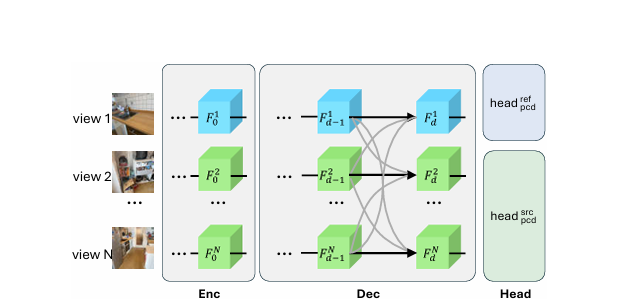
\includegraphics[width=0.95\linewidth]{Figure1.png}
    \caption{Tổng quan kiến trúc \mvd{}/\mvdp{} trích từ \cite{mvdust3r_paper}. Hình này minh họa cách mô hình nhận nhiều ảnh RGB, mã hóa chúng thành visual tokens, trao đổi thông tin qua decoder và dự đoán các pointmap 3D.}
    \label{fig:mvdust3r_overview}
\end{figure}

Về mặt kiến trúc, \mvdp{} có thể được chia thành bốn thành phần chính.

\textbf{Encoder ảnh.} Mỗi ảnh RGB $I^v$ được đưa qua một ViT encoder dùng chung trọng số:
\begin{equation}
F_0^v = Enc(I^v).
\end{equation}
Encoder biến ảnh 2D thành một chuỗi visual tokens. Các token này chứa đặc trưng thị giác ban đầu như cạnh, texture, vùng phẳng, vật thể, bố cục không gian và các dấu hiệu hình học gián tiếp từ ảnh RGB.

\textbf{Multi-view decoder blocks.} Sau encoder, các view không còn được xử lý độc lập. Trong mỗi decoder block, một view đang được cập nhật đóng vai trò primary view, còn các view còn lại đóng vai trò secondary views. Decoder thực hiện self-attention trên primary tokens, sau đó dùng cross-attention để lấy thông tin từ tokens của các view khác. Nhờ vậy, mô hình có thể dùng bằng chứng hình học từ nhiều góc nhìn thay vì chỉ suy luận từ một cặp ảnh.

\textbf{Multi-path reference-view structure.} Bản \mvd{} cơ sở dùng một reference view duy nhất. Điều này có thể gây khó khăn trong scene lớn, vì một reference view thường không có overlap tốt với tất cả source views. \mvdp{} khắc phục bằng cách chọn nhiều reference views:
\begin{equation}
R = \{r^m\}_{m=1}^{M}.
\end{equation}
Mỗi reference view tạo ra một path riêng. Trong path thứ $m$, tất cả pointmap được dự đoán trong hệ tọa độ của reference view $r^m$.

\begin{figure}[H]
    \centering
    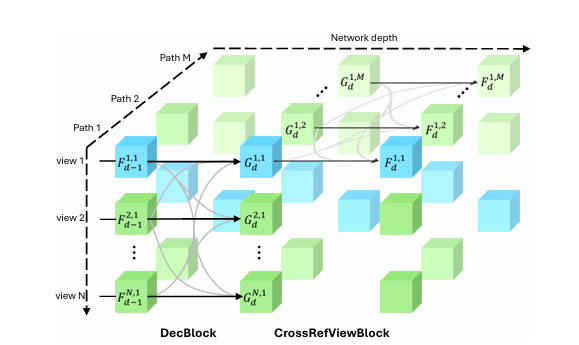
\includegraphics[width=0.95\linewidth]{Figure2.png}
    \caption{Cấu trúc nhiều reference paths và Cross-Reference-View Block của \mvdp{} trích từ \cite{mvdust3r_paper}. Các DecBlock trao đổi thông tin giữa nhiều view trong cùng một path, còn CrossRefViewBlock trao đổi thông tin của cùng một view qua nhiều reference paths khác nhau.}
    \label{fig:crossref_block}
\end{figure}

\textbf{Cross-Reference-View Block.} Đây là điểm mở rộng quan trọng của \mvdp{}. Sau mỗi DecBlock, mô hình không chỉ fuse thông tin giữa các view trong cùng một path mà còn fuse thông tin của cùng một view qua nhiều reference paths khác nhau. Với view $v$ và reference path $m$, mô hình có intermediate representation $G_d^{v,m}$. Cross-Reference-View Block cập nhật representation này bằng cách nhìn sang representation của cùng view $v$ trong các path còn lại:
\begin{equation}
F_d^{v,m}=CrossRefViewBlock_d(G_d^{v,m},G_d^{v,-m}).
\end{equation}
Nếu một view khó được dựng tốt trong path thứ nhất nhưng lại được dựng tốt hơn trong path thứ hai, block này cho phép thông tin tốt hơn được truyền sang các path khác. Vì vậy, \mvdp{} giảm phụ thuộc vào một reference view duy nhất và ổn định hơn trong scene lớn hoặc sparse-view có viewpoint change mạnh.

\textbf{Pointmap head và confidence map.} Sau nhiều decoder layers, các regression heads dự đoán pointmap và confidence map. Với mỗi view, đầu ra gồm:
\begin{equation}
X^{v,m}\in \mathbb{R}^{H\times W\times 3}, \qquad C^{v,m}\in \mathbb{R}^{H\times W}.
\end{equation}
$X^{v,m}$ là pointmap 3D, còn $C^{v,m}$ là confidence map biểu thị mức độ tin cậy của mô hình tại từng pixel. Trong dự án này, pointmap đầu ra được chuyển thành point cloud ban đầu. Point cloud này được xem là candidate geometry, tức là một đề xuất hình học ban đầu có thể cần được kiểm tra và hiệu chỉnh bằng depth map ước lượng.

\subsection{Kiến trúc mô hình ước lượng độ sâu Depth Anything V2 Metric Indoor}
Mô hình thứ hai trong pipeline là \da{} Metric Indoor. Đây là mô hình monocular depth estimation: nó nhận một ảnh RGB đơn lẻ và dự đoán một depth map dày đặc cho ảnh đó. Với mỗi ảnh đầu vào:
\begin{equation}
I^v \in \mathbb{R}^{H\times W\times 3},
\end{equation}
mô hình dự đoán:
\begin{equation}
\hat{D}^{v}\in \mathbb{R}^{H\times W}.
\end{equation}
Mỗi giá trị $\hat{D}^{v}(p)$ biểu diễn độ sâu ước lượng tại pixel $p$. Với bản Metric Indoor, mô hình được fine-tune để depth có ý nghĩa theo thang đo metric trong không gian indoor, thay vì chỉ biểu diễn thứ tự gần--xa tương đối.


\begin{figure}[H]
\centering
\resizebox{0.95\linewidth}{!}{%
\begin{tikzpicture}[
    node distance=0.9cm and 1.0cm,
    box/.style={draw, rounded corners, align=center, minimum width=2.8cm, minimum height=0.9cm, fill=blue!5},
    proc/.style={draw, rounded corners, align=center, minimum width=2.9cm, minimum height=0.9cm, fill=green!8},
    outbox/.style={draw, rounded corners, align=center, minimum width=2.9cm, minimum height=0.9cm, fill=orange!12},
    arr/.style={-{Latex[length=3mm]}, thick}
]
\node[box] (rgb) {Ảnh RGB\\$I^v$};
\node[proc, right=of rgb] (enc) {DINOv2/ViT\\encoder};
\node[proc, right=of enc] (dec) {DPT\\decoder};
\node[proc, below=of dec] (head) {Depth\\prediction head};
\node[outbox, left=of head] (depth) {Depth map\\$\hat{D}^{v}$};
\draw[arr] (rgb) -- (enc);
\draw[arr] (enc) -- (dec);
\draw[arr] (dec) -- (head);
\draw[arr] (head) -- (depth);
\end{tikzpicture}%
}
\caption{Luồng xử lý của mô hình ước lượng độ sâu monocular trong dự án. Mỗi ảnh RGB được xử lý độc lập qua encoder, decoder và depth head để tạo depth map ước lượng. Sơ đồ được bố trí thành hai hàng để không vượt quá lề trang.}
\label{fig:depth_estimator}
\end{figure}

Có thể hiểu kiến trúc \da{} Metric Indoor theo ba khối chính. \textbf{Image encoder} sử dụng backbone dạng Vision Transformer dựa trên DINOv2 để trích xuất đặc trưng từ ảnh RGB. \textbf{DPT decoder} kết hợp đặc trưng ở nhiều tầng để phục hồi thông tin không gian dày đặc. \textbf{Depth prediction head} biến feature map sau decoder thành depth map:
\begin{equation}
\hat{D}^{v}=DepthHead(Decoder(Encoder(I^v))).
\end{equation}

Trong project, mô hình depth estimation không trực tiếp tạo point cloud cuối cùng. Thay vào đó, nó cung cấp một depth prior cho từng source view. Depth map này được dùng để kiểm tra xem candidate 3D points do \mvdp{} tạo ra có phù hợp với độ sâu quan sát được trong từng ảnh hay không. Nếu một candidate point khi project về một source view có depth khác biệt lớn so với depth map ước lượng, điểm đó có thể bị xem là không nhất quán hình học và cần được loại bỏ hoặc hiệu chỉnh.

\subsection{Quan hệ giữa hai mô hình trong pipeline}
Hai mô hình có vai trò bổ sung cho nhau. \mvdp{} khai thác quan hệ multi-view giữa nhiều ảnh RGB để tạo candidate 3D geometry. Nó mạnh ở chỗ có thể suy luận hình học scene từ nhiều view mà không cần pose camera làm input bắt buộc. Tuy nhiên, vì reconstruction ban đầu dựa trên RGB-only, một số candidate points có thể bị sai ở vùng occlusion, vùng có vật thể lặp lại, vùng ít texture hoặc vùng có viewpoint change lớn.

Ngược lại, \da{} Metric Indoor không xử lý nhiều view cùng lúc. Nó dự đoán depth từ từng ảnh đơn lẻ. Vì chỉ dùng một ảnh, depth estimator không thể tự giải quyết hoàn toàn mọi mơ hồ hình học của monocular depth estimation. Tuy nhiên, nó cung cấp một tín hiệu depth độc lập với backbone multi-view. Khi kết hợp hai mô hình, pipeline có thể dùng depth map để kiểm tra, lọc hoặc hiệu chỉnh candidate geometry từ \mvdp{}.

Có thể tóm tắt luồng xử lý như sau:
\begin{equation}
\{I^v\}_{v=1}^{N}\xrightarrow{\ \mvdp{}\ }\{X^v,C^v\}_{v=1}^{N}\xrightarrow{}\text{candidate point cloud},
\end{equation}
đồng thời với từng ảnh:
\begin{equation}
I^v\xrightarrow{\ \da{}\ }\hat{D}^{v}.
\end{equation}
Sau đó, candidate points từ \mvdp{} được kiểm tra bằng các depth maps $\{\hat{D}^{v}\}$ để tạo ra geometry đã được hiệu chỉnh hoặc lọc bỏ các điểm không nhất quán.

% ------------------------------------------------------------------
\section{Dataset}
Dự án này sử dụng một dataset RGB-D theo phong cách ScanNet có kiểm soát để hỗ trợ cả giám sát độ sâu và đánh giá tái dựng 3D. ScanNet là một RGB-D video dataset chứa hàng triệu view, camera poses, surface reconstructions và semantic annotations trên hơn 1500 scans \cite{scannet}. Việc có sẵn ảnh RGB, depth maps và camera geometry khiến dataset này phù hợp để huấn luyện và đánh giá các phương pháp tái dựng có hỗ trợ bởi độ sâu.

\subsection{Chiến lược lựa chọn dataset}
Dataset được dùng theo hai cách khác nhau. Thứ nhất, ảnh RGB được dùng làm modality đầu vào tại thời điểm triển khai. Thứ hai, depth maps và camera poses được dùng trong huấn luyện và đánh giá. Sự phân biệt này rất quan trọng. Dự án không tuyên bố rằng sản phẩm cuối cần depth maps. Thay vào đó, nó dùng depth trong dataset làm tín hiệu huấn luyện cho bộ ước lượng độ sâu và làm tham chiếu để đánh giá reconstructed point clouds.

Thiết kế này xuất phát từ động lực thực tế của dự án. Trong sử dụng đời thực, phần lớn người dùng có ảnh RGB nhưng không có depth maps. Một dataset có nhãn RGB-D vì vậy có giá trị vì nó cho phép hệ thống học các prior hình học trước khi triển khai. Sau khi được huấn luyện, bộ ước lượng độ sâu có thể dự đoán pseudo-depth từ ảnh RGB, từ đó cho phép hiệu chỉnh có hướng dẫn bởi độ sâu mà không cần cảm biến chiều sâu vật lý.

\subsection{Dữ liệu RGB-D cho giám sát}
Với mỗi scene, dataset cung cấp RGB frames, depth maps và thông tin camera. Trong quá trình fine-tuning bộ ước lượng độ sâu, ảnh RGB được dùng làm đầu vào và depth map đo tương ứng được dùng làm giám sát. Gọi $I_i$ là ảnh RGB và $D_i$ là depth map đo trực tiếp của nó. Bộ ước lượng độ sâu $F_\theta$ dự đoán:
\begin{equation}
\hat{D}_i = F_\theta(I_i),
\end{equation}
trong đó $\hat{D}_i$ là depth map ước lượng. Mục tiêu huấn luyện khuyến khích $\hat{D}_i$ gần với $D_i$ trên các pixel hợp lệ.

\subsection{Xây dựng nhóm sparse-view}
Giai đoạn tái dựng chỉ sử dụng một số lượng nhỏ ảnh RGB từ mỗi scene. Một nhóm sparse-view chứa $N$ views:
\begin{equation}
\mathcal{V}=\{I_1,I_2,\ldots,I_N\}, \qquad N \in \{3,4,5\}.
\end{equation}
Thiết kế này biểu diễn một tình huống thực tế trong đó người dùng chỉ cung cấp vài bức ảnh thay vì một chuỗi video đầy đủ.

Các nhóm view được chọn được giữ cố định giữa các phương pháp so sánh. Điều này bảo đảm rằng khác biệt hiệu năng đến từ phương pháp tái dựng, không đến từ việc chọn đầu vào khác nhau. Vì vậy, báo cáo đánh giá tái dựng trong một setting sparse-view được chọn có kiểm soát, không phải bài toán automatic view selection.

\subsection{Tiền xử lý dữ liệu}
Ảnh RGB được resize hoặc crop theo yêu cầu đầu vào của \mvdp{} và bộ ước lượng độ sâu. Depth maps được lọc để loại bỏ các pixel không hợp lệ và chỉ được dùng cho giám sát và đánh giá. Khi huấn luyện bộ ước lượng độ sâu, các phép augmentation chuẩn như resize, crop và flip có thể được áp dụng nhất quán cho cặp RGB-depth để giữ đúng căn chỉnh.

Điểm quan trọng là bước preprocessing phải giữ nguyên ràng buộc suy luận chỉ dùng RGB. Mọi thao tác sử dụng depth measured đều thuộc giai đoạn training hoặc evaluation. Không có depth measured nào được đưa vào mô hình cuối tại deployment time.

% ------------------------------------------------------------------
\section{Phương pháp}
\subsection{Tổng quan pipeline được đề xuất}
Hình~\ref{fig:pipeline} minh họa pipeline được đề xuất. Hệ thống nhận một tập nhỏ ảnh RGB. Nhánh thứ nhất dùng \mvdp{} để dự đoán các 3D pointmap ứng viên. Nhánh thứ hai dùng bộ ước lượng độ sâu monocular đã tinh chỉnh để dự đoán pseudo-depth maps từ chính các ảnh RGB đó. Các depth maps ước lượng sau đó được dùng để hiệu chỉnh candidate geometry, tạo ra point cloud cuối cùng.

\begin{figure}[H]
\centering
\resizebox{0.98\linewidth}{!}{%
\begin{tikzpicture}[
    box/.style={draw, rounded corners, align=center, minimum width=3.1cm, minimum height=1.05cm, fill=blue!5},
    proc/.style={draw, rounded corners, align=center, minimum width=3.7cm, minimum height=1.05cm, fill=green!8},
    corrbox/.style={draw, rounded corners, align=center, minimum width=3.2cm, minimum height=1.05cm, fill=yellow!12},
    outbox/.style={draw, rounded corners, align=center, minimum width=3.1cm, minimum height=1.05cm, fill=orange!12},
    arr/.style={-{Latex[length=3mm]}, thick}
]
\node[box] (input) at (0,0) {Các view RGB thưa\\$I_1,\ldots,I_N$};
\node[proc] (mvd) at (4.4,1.0) {\mvdp{}\\candidate pointmaps};
\node[proc] (depth) at (4.4,-1.0) {Bộ ước lượng độ sâu\\đã tinh chỉnh\\depth maps ước lượng};
\node[corrbox] (corr) at (8.8,0) {Hiệu chỉnh bằng\\độ sâu ước lượng};
\node[outbox] (outnode) at (12.7,0) {Point cloud\\3D cuối cùng};
\draw[arr] (input.east) -- (mvd.west);
\draw[arr] (input.east) -- (depth.west);
\draw[arr] (mvd.east) -- (corr.north west);
\draw[arr] (depth.east) -- (corr.south west);
\draw[arr] (corr.east) -- (outnode.west);
\end{tikzpicture}%
}
\caption{Tổng quan pipeline tái dựng sparse-view chỉ dùng RGB được đề xuất. Nhánh \mvdp{} tạo candidate pointmaps, nhánh depth estimator tạo depth maps ước lượng, sau đó module correction kết hợp hai nguồn thông tin để tạo point cloud cuối cùng.}
\label{fig:pipeline}
\end{figure}

Pipeline có thể được viết như sau:
\begin{equation}
P_{\text{cand}} = F_{\text{MV}}(I_1,\ldots,I_N),
\end{equation}
\begin{equation}
\hat{D}_i = F_\theta(I_i), \qquad i=1,\ldots,N,
\end{equation}
\begin{equation}
P_{\text{final}} = C(P_{\text{cand}}, \hat{D}_1,\ldots,\hat{D}_N),
\end{equation}
trong đó $F_{\text{MV}}$ là backbone \mvdp{}, $F_\theta$ là bộ ước lượng độ sâu đã tinh chỉnh, và $C(\cdot)$ là module hiệu chỉnh bằng độ sâu ước lượng.

\subsection{Candidate geometry từ MV-DUSt3R+}
Nhánh \mvdp{} dự đoán các candidate pointmaps multi-view từ ảnh RGB. Các pointmap này cung cấp ước lượng ban đầu về hình học của scene. Nhánh này quan trọng vì nó lập luận qua nhiều view thay vì ước lượng độ sâu độc lập cho từng ảnh.

Tuy nhiên, candidate point cloud có thể chứa các điểm sai độ sâu. Những lỗi như vậy có thể xuất hiện ở vùng ít texture, cấu trúc lặp lại, vùng bị che khuất và các view có độ chồng lấp yếu. Do đó, candidate geometry được xem là một đề xuất hình học mạnh nhưng chưa hoàn hảo.

\subsection{Ước lượng độ sâu monocular đã tinh chỉnh}
Nhánh độ sâu ước lượng một depth map từ mỗi ảnh RGB. Một mô hình độ sâu pretrained như \da{} được dùng làm khởi tạo. Sau đó, mô hình được fine-tune trên các scene huấn luyện bằng cách dùng độ sâu đo trực tiếp làm giám sát. Mục đích của fine-tuning là thích nghi bộ ước lượng độ sâu với hình học trong nhà và giảm lỗi metric-scale.

Với các pixel độ sâu hợp lệ $\Omega$, một depth loss đơn giản có thể được viết là:
\begin{equation}
\mathcal{L}_{\text{depth}} = \frac{1}{|\Omega|}\sum_{p\in\Omega}|\hat{D}(p)-D(p)|.
\end{equation}
Các loss bổ sung như scale-invariant depth loss, gradient loss hoặc smoothness regularization có thể được thêm nếu cần:
\begin{equation}
\mathcal{L}_{\text{total}} = \lambda_1\mathcal{L}_{\text{depth}} + \lambda_2\mathcal{L}_{\text{grad}} + \lambda_3\mathcal{L}_{\text{smooth}}.
\end{equation}
Báo cáo cuối có thể cập nhật các thành phần loss chính xác theo training script đã triển khai.

\subsection{Hiệu chỉnh bằng độ sâu ước lượng}
Module correction dùng estimated depth như một neo hình học. Với một candidate point gắn với source pixel $p=(u,v)$, giá trị độ sâu dự đoán $\hat{D}(p)$ được back-project thành một điểm 3D:
\begin{equation}
X_{\text{depth}} = \hat{D}(p)K^{-1}\begin{bmatrix}u\\v\\1\end{bmatrix},
\end{equation}
trong đó $K$ là ma trận camera intrinsic nếu có trong setting đánh giá. Bước correction so sánh candidate point $X_{\text{cand}}$ với estimated-depth point $X_{\text{depth}}$:
\begin{equation}
r = \|X_{\text{cand}}-X_{\text{depth}}\|_2.
\end{equation}
Nếu residual $r$ lớn nhưng độ sâu ước lượng được xem là đáng tin cậy, candidate point được kéo về phía estimated-depth anchor:
\begin{equation}
X_{\text{corr}} = (1-\alpha)X_{\text{cand}} + \alpha X_{\text{depth}},
\end{equation}
trong đó $\alpha \in [0,1]$ điều khiển cường độ hiệu chỉnh. Thiết kế này giữ lại prior multi-view từ \mvdp{} đồng thời dùng độ sâu ước lượng để giảm lỗi wrong-depth.

\subsection{Khác biệt so với backprojection trực tiếp từ depth}
Phương pháp được đề xuất khác với việc trực tiếp chuyển estimated depth maps thành point clouds. Backprojection trực tiếp chỉ dùng bộ ước lượng độ sâu để tạo hình học. Ngược lại, phương pháp được đề xuất vẫn giữ \mvdp{} làm backbone tái dựng multi-view và chỉ dùng estimated depth để hiệu chỉnh candidate geometry. Điều này cho phép pipeline kết hợp lập luận RGB multi-view với depth priors đã học.

% ------------------------------------------------------------------
\section{Thí nghiệm và kết quả}
\subsection{Thiết lập thí nghiệm}
Thiết lập thí nghiệm đi theo bản chất hai giai đoạn của dự án. Thứ nhất, bộ ước lượng độ sâu được huấn luyện hoặc tinh chỉnh bằng giám sát RGB-D từ training split. Thứ hai, pipeline tái dựng được đánh giá với đầu vào chỉ là RGB tại thời điểm suy luận. Độ sâu đo trực tiếp được dùng để tính reference geometry và các metric đánh giá, nhưng không được đưa vào phương pháp cuối như một đầu vào.

Các phương pháp so sánh được tóm tắt trong Bảng~\ref{tab:methods}.
\begin{table}[H]
\centering
\renewcommand{\arraystretch}{1.2}
\begin{tabular}{p{0.28\linewidth}p{0.19\linewidth}p{0.18\linewidth}p{0.25\linewidth}}
\toprule
Phương pháp & Đầu vào RGB & Độ sâu đo trực tiếp khi suy luận & Mục đích \\
\midrule
RGB-only \mvdp{} & Có & Không & Backbone tái dựng multi-view baseline \\
Backprojection trực tiếp từ độ sâu ước lượng & Có & Không & Kiểm tra liệu chỉ độ sâu dự đoán có đủ hay không \\
Hiệu chỉnh bằng độ sâu pretrained & Có & Không & Kiểm tra prior độ sâu off-the-shelf \\
Hiệu chỉnh bằng độ sâu ước lượng đã tinh chỉnh (Ours) & Có & Không & Setting sản phẩm chính được đề xuất \\
\bottomrule
\end{tabular}
\caption{Các phương pháp so sánh. Tất cả các biến thể tại thời điểm triển khai chỉ dùng đầu vào RGB. Độ sâu đo trực tiếp được dùng cho huấn luyện và đánh giá, không dùng làm đầu vào suy luận.}
\label{tab:methods}
\end{table}

\subsection{Các metric đánh giá}
Chúng tôi đánh giá framework được đề xuất từ hai góc nhìn: chất lượng monocular depth estimation và chất lượng tái dựng 3D downstream. Thiết kế này phản ánh bản chất hai giai đoạn của dự án. Bộ ước lượng độ sâu trước hết phải dự đoán được thông tin hình học hữu ích từ ảnh RGB, sau đó reconstructed point cloud phải cải thiện so với baseline multi-view chỉ dùng RGB.

\subsubsection{Metric cho ước lượng độ sâu}
Đối với ước lượng độ sâu, gọi $D$ là độ sâu tham chiếu đo trực tiếp và $\hat{D}$ là độ sâu dự đoán. Các metric chỉ được tính trên tập pixel hợp lệ $\Omega$.

\textbf{Absolute Relative Error (AbsRel).} AbsRel đo lỗi độ sâu tương đối được chuẩn hóa bởi ground-truth depth:
\begin{equation}
\mathrm{AbsRel} = \frac{1}{|\Omega|}\sum_{p\in\Omega} \frac{|\hat{D}(p)-D(p)|}{D(p)}.
\end{equation}
AbsRel thấp hơn cho thấy độ sâu dự đoán gần hơn với độ sâu đo trực tiếp theo relative scale.

\textbf{Mean Absolute Error (MAE).} MAE đo lỗi độ sâu tuyệt đối trung bình theo mét:
\begin{equation}
\mathrm{MAE}=\frac{1}{|\Omega|}\sum_{p\in\Omega}|\hat{D}(p)-D(p)|.
\end{equation}
Metric này dễ diễn giải vì nó trực tiếp báo cáo lỗi depth theo đơn vị mét.

\textbf{Root Mean Squared Error (RMSE).} RMSE phạt mạnh hơn đối với các lỗi độ sâu lớn:
\begin{equation}
\mathrm{RMSE}=\sqrt{\frac{1}{|\Omega|}\sum_{p\in\Omega}(\hat{D}(p)-D(p))^2}.
\end{equation}
RMSE cao so với MAE cho thấy mô hình có thể có các outlier errors lớn.

\textbf{Threshold accuracy.} Các metric $\delta$ đo tỉ lệ pixel có độ sâu dự đoán nằm trong một ngưỡng nhân so với độ sâu tham chiếu:
\begin{equation}
\delta_k = \frac{|\{p\in\Omega: \max(\frac{\hat{D}(p)}{D(p)},\frac{D(p)}{\hat{D}(p)}) < 1.25^k\}|}{|\Omega|}, \quad k\in\{1,2,3\}.
\end{equation}
$\delta_1$, $\delta_2$ và $\delta_3$ càng cao thì chất lượng dự đoán độ sâu càng tốt.

\textbf{Scale-aligned error.} Vì monocular depth estimation chịu scale ambiguity, chúng tôi cũng đánh giá depth sau khi áp dụng một hệ số căn chỉnh vô hướng $s$:
\begin{equation}
D_{\text{aligned}} = s\hat{D}.
\end{equation}
Aligned MAE và RMSE đo xem dự đoán có cấu trúc tương đối hữu ích hay không, ngay cả khi raw metric scale chưa hoàn hảo.

\subsubsection{Metric cho tái dựng 3D}
Đối với tái dựng 3D, gọi $P$ là predicted point cloud và $G$ là proxy ground-truth point cloud. Khoảng cách từ một điểm $p$ đến point cloud $G$ được định nghĩa là:
\begin{equation}
d(p,G)=\min_{g\in G}\|p-g\|_2.
\end{equation}

\textbf{Accuracy.} Accuracy đo mức độ gần của predicted points với reference geometry:
\begin{equation}
\mathrm{Accuracy}=\frac{1}{|P|}\sum_{p\in P}d(p,G).
\end{equation}
Giá trị thấp hơn cho thấy ít floating points hoặc các điểm dự đoán bị đặt sai vị trí hơn.

\textbf{Completeness.} Completeness đo mức độ point cloud dự đoán bao phủ reference geometry:
\begin{equation}
\mathrm{Completeness}=\frac{1}{|G|}\sum_{g\in G}d(g,P).
\end{equation}
Giá trị thấp hơn cho thấy ít vùng bị thiếu hơn.

\textbf{Precision và Recall.} Với một ngưỡng khoảng cách $\tau$, precision đo tỉ lệ predicted points gần reference geometry, trong khi recall đo tỉ lệ reference points được bao phủ bởi prediction:
\begin{equation}
\mathrm{Precision@}\tau=\frac{|\{p\in P:d(p,G)<\tau\}|}{|P|},
\end{equation}
\begin{equation}
\mathrm{Recall@}\tau=\frac{|\{g\in G:d(g,P)<\tau\}|}{|G|}.
\end{equation}
Trong dự án này, $\tau=0.05$ m được dùng khi báo cáo precision và recall ở ngưỡng 5 cm.

\textbf{F-score.} F-score là trung bình điều hòa của precision và recall:
\begin{equation}
F_1=\frac{2\cdot\mathrm{Precision}\cdot\mathrm{Recall}}{\mathrm{Precision}+\mathrm{Recall}}.
\end{equation}
F-score cao đòi hỏi reconstruction vừa chính xác vừa đủ hoàn chỉnh.

\textbf{Chamfer distance.} Chamfer distance kết hợp hai khoảng cách nearest-neighbor theo hai chiều:
\begin{equation}
\mathrm{Chamfer}=\mathrm{Accuracy}+\mathrm{Completeness}.
\end{equation}
Chamfer distance thấp hơn cho thấy mức độ khớp hình học tổng thể tốt hơn.

\textbf{Normalized Distance và DAc.} Để so sánh chất lượng hình dạng sau khi loại bỏ khác biệt scale và tâm toàn cục, point cloud có thể được chuẩn hóa trước khi đánh giá. Normalized Distance (ND) đo khoảng cách nearest-neighbor trung bình sau chuẩn hóa, và DAc@$0.2$ đo tỉ lệ điểm nằm trong một ngưỡng khoảng cách đã chuẩn hóa. Các metric này hữu ích để phân tích chất lượng ở mức shape, nhưng không nên diễn giải chúng như các metric đo pose hoặc scale tuyệt đối theo hệ mét.

\subsection{Đánh giá ước lượng độ sâu}
Đánh giá ước lượng độ sâu kiểm tra xem bộ ước lượng độ sâu đã tinh chỉnh có đủ chính xác để đóng vai trò là correction anchor hay không. Các số trong Bảng~\ref{tab:depthtrain} và Bảng~\ref{tab:depthmetrics} được lấy từ Run 37. Checkpoint dùng để báo cáo held-out là \texttt{controlled\_best}. Checkpoint \texttt{full\_dataset\_deployment} chỉ là artifact triển khai vì nó được huấn luyện lại trên toàn bộ frame đã phát hiện.

\begin{table}[H]
\centering
\small
\renewcommand{\arraystretch}{1.18}
\resizebox{\linewidth}{!}{%
\begin{tabular}{@{}lrrrrrr@{}}
\toprule
Giai đoạn & Số scene & Số frame dùng huấn luyện & Epoch & Mini-batch step & Train loss trung bình & Runtime \\
\midrule
Controlled train split & 1210 & 198862 & 1 & 99431 & 0.0850 & 4.01 giờ \\
Full-data deployment & 1513 & 248402 & 1 & 124201 & 0.0718 & 4.08 giờ \\
\bottomrule
\end{tabular}%
}
\caption{Workload fine-tuning của depth estimator trong Run 37. Giai đoạn controlled dùng train split để chọn checkpoint \texttt{controlled\_best}; giai đoạn full-data deployment dùng toàn bộ scene đã phát hiện để tạo checkpoint triển khai.}
\label{tab:depthtrain}
\end{table}

\begin{table}[H]
\centering
\small
\renewcommand{\arraystretch}{1.18}
\resizebox{\linewidth}{!}{%
\begin{tabular}{@{}lcccccc@{}}
\toprule
Mô hình độ sâu & AbsRel $\downarrow$ & MAE (m) $\downarrow$ & RMSE (m) $\downarrow$ & $\delta_1$ $\uparrow$ & Scale-aligned MAE $\downarrow$ & Split \\
\midrule
Pretrained \da{} Metric Indoor & 0.2730 & 0.3839 & 0.4778 & 0.6441 & 0.1672 & validation \\
Fine-tuned \texttt{controlled\_best} & \textbf{0.1145} & \textbf{0.1431} & \textbf{0.2393} & \textbf{0.9355} & \textbf{0.0992} & validation \\
Pretrained \da{} Metric Indoor & 0.2707 & 0.3850 & 0.4806 & 0.6486 & 0.1676 & test \\
Fine-tuned \texttt{controlled\_best} & \textbf{0.1140} & \textbf{0.1428} & \textbf{0.2370} & \textbf{0.9362} & \textbf{0.0982} & test \\
\bottomrule
\end{tabular}%
}
\caption{Đánh giá ước lượng độ sâu trên held-out frames của Run 37. Mỗi split dùng 1200 frames lấy từ các scene held-out; validation gồm 149 scene và test gồm 152 scene.}
\label{tab:depthmetrics}
\end{table}

Kết quả cho thấy fine-tuning làm giảm mạnh lỗi depth. Trên validation, AbsRel giảm từ 0.2730 xuống 0.1145, MAE giảm từ 0.3839 m xuống 0.1431 m và $\delta_1$ tăng từ 0.6441 lên 0.9355. Trên test, AbsRel giảm từ 0.2707 xuống 0.1140, MAE giảm từ 0.3850 m xuống 0.1428 m và $\delta_1$ tăng từ 0.6486 lên 0.9362. Điều này cho thấy depth estimator sau fine-tuning đáng tin cậy hơn nhiều so với checkpoint pretrained ban đầu trong controlled ScanNet-style indoor subset.

\begin{figure}[H]
    \centering
    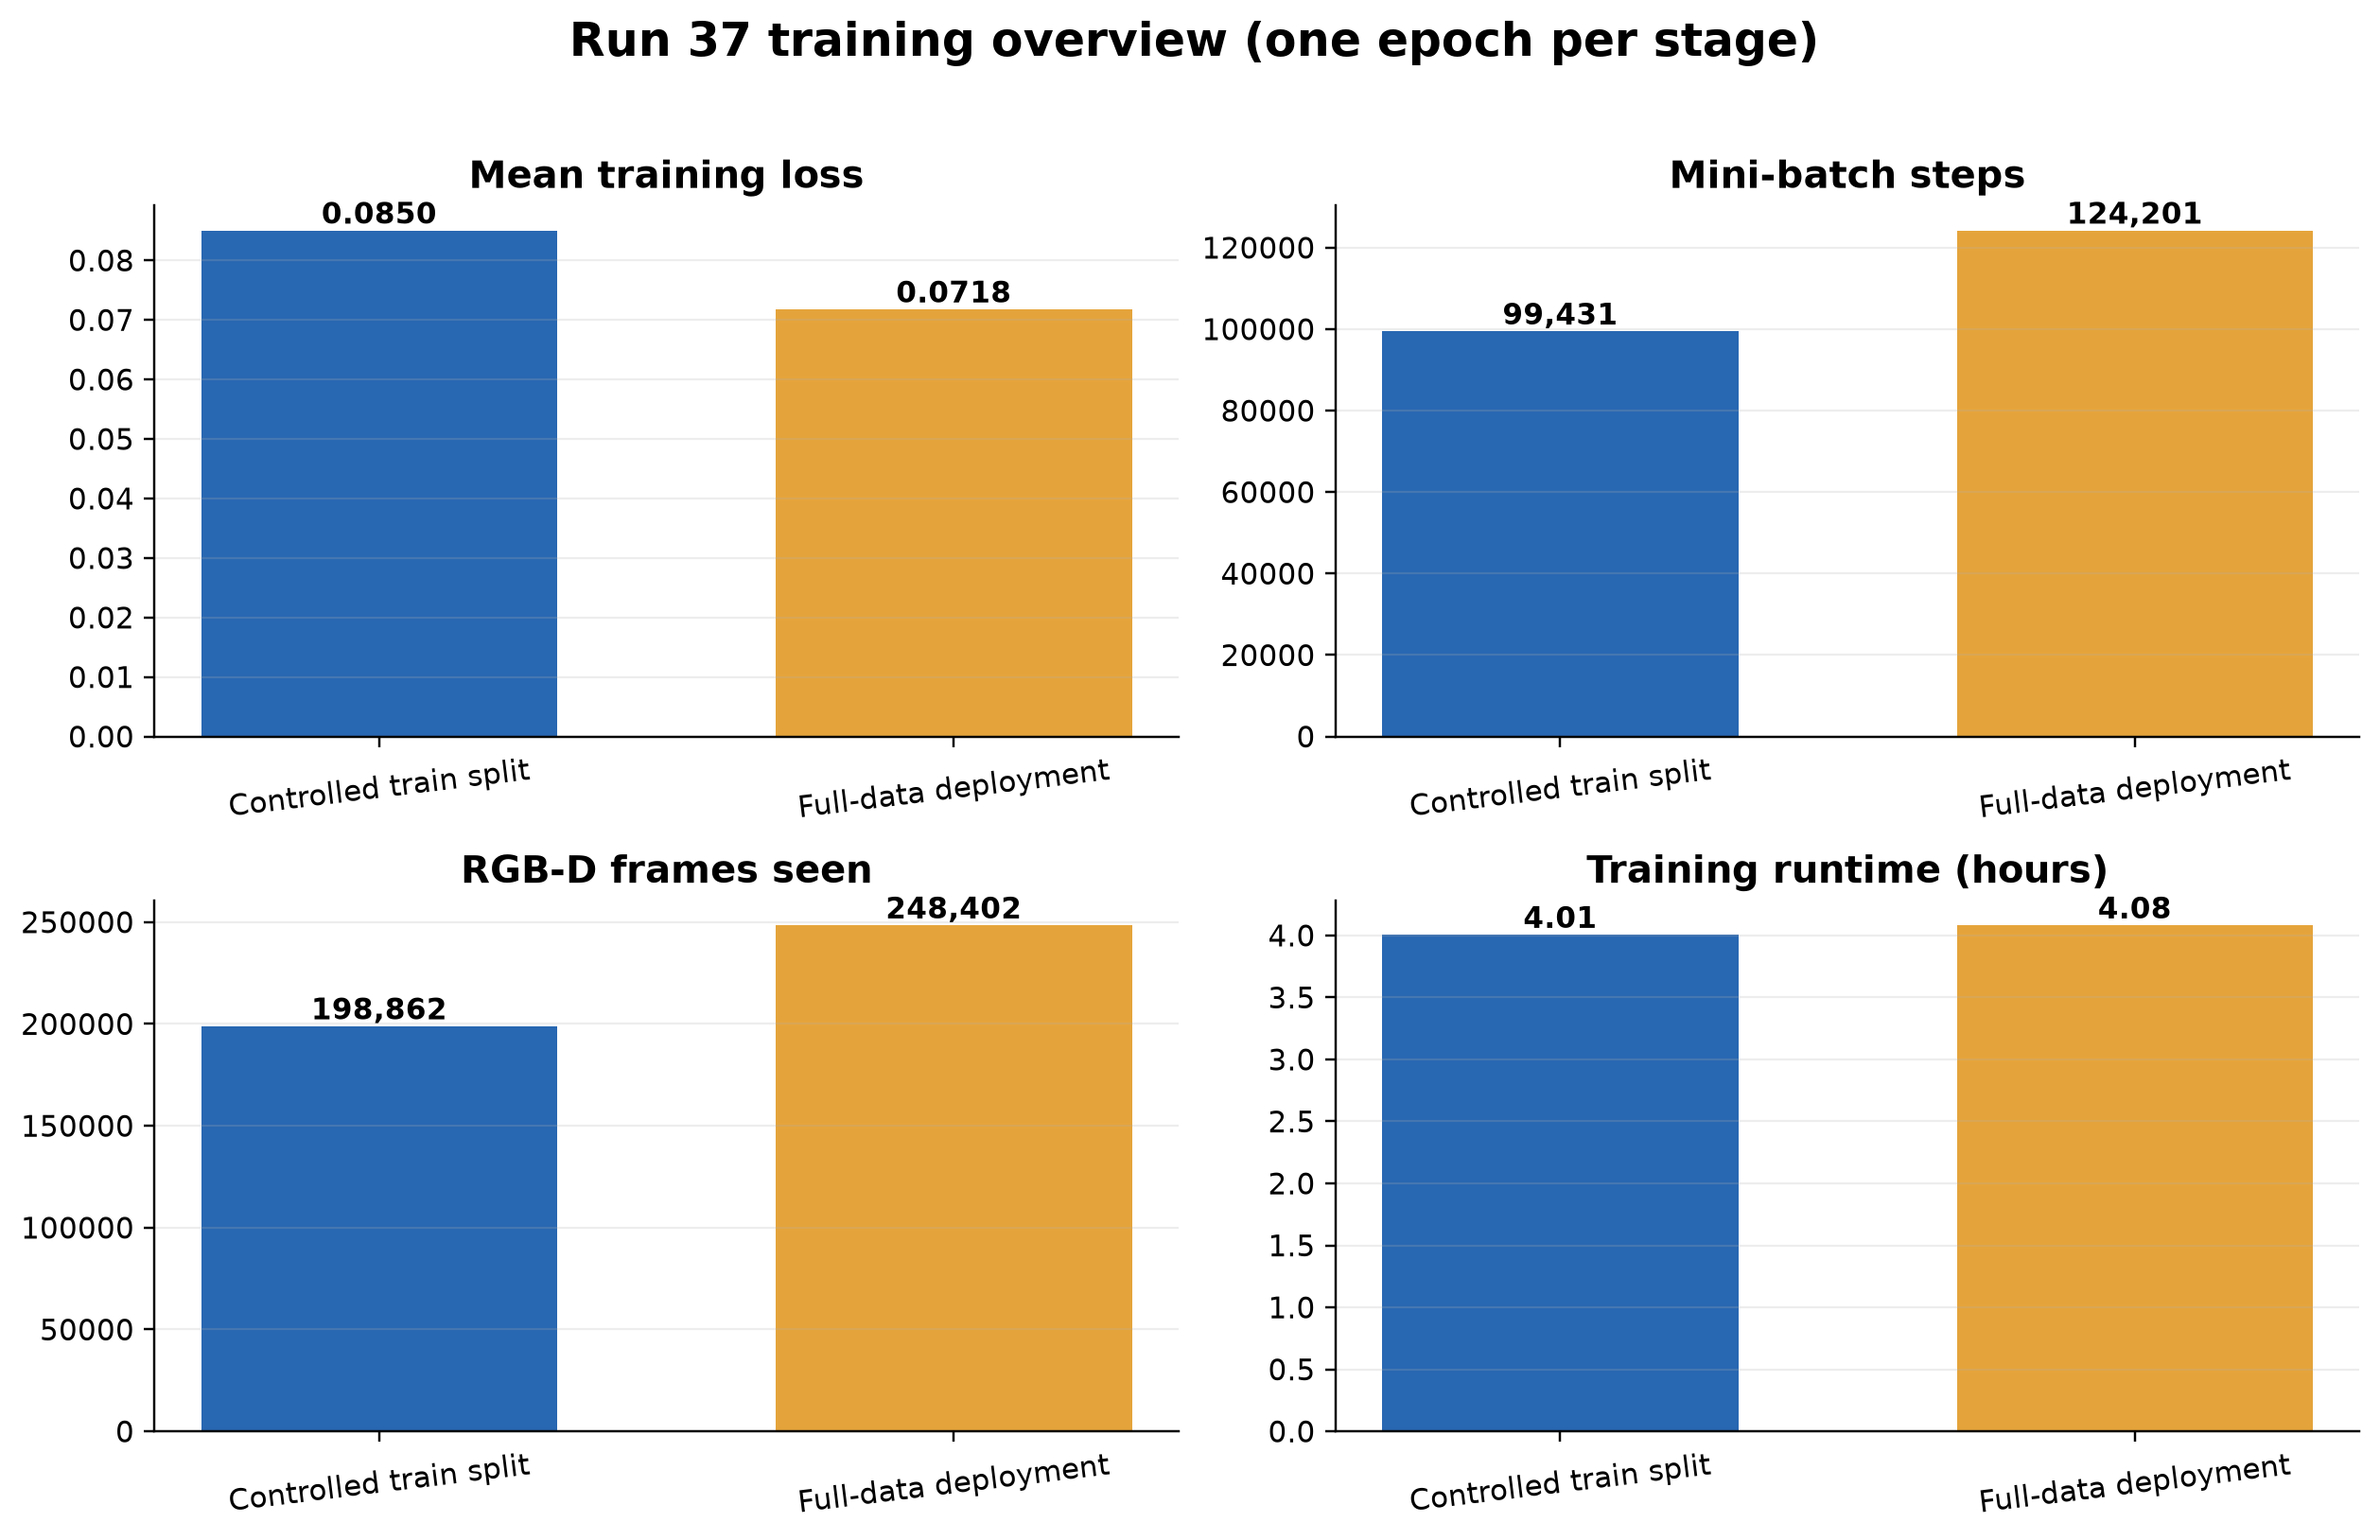
\includegraphics[width=0.92\linewidth]{Run37_training_overview.png}
    \caption{Tổng quan workload fine-tuning trong Run 37. Vì Run 37 chỉ log một epoch cho mỗi giai đoạn, hình này không được diễn giải như một training-loss curve nhiều epoch mà là tổng kết workload, loss trung bình và runtime.}
    \label{fig:run37_training_overview}
\end{figure}

\begin{figure}[H]
    \centering
    \begin{subfigure}{0.96\linewidth}
        \centering
        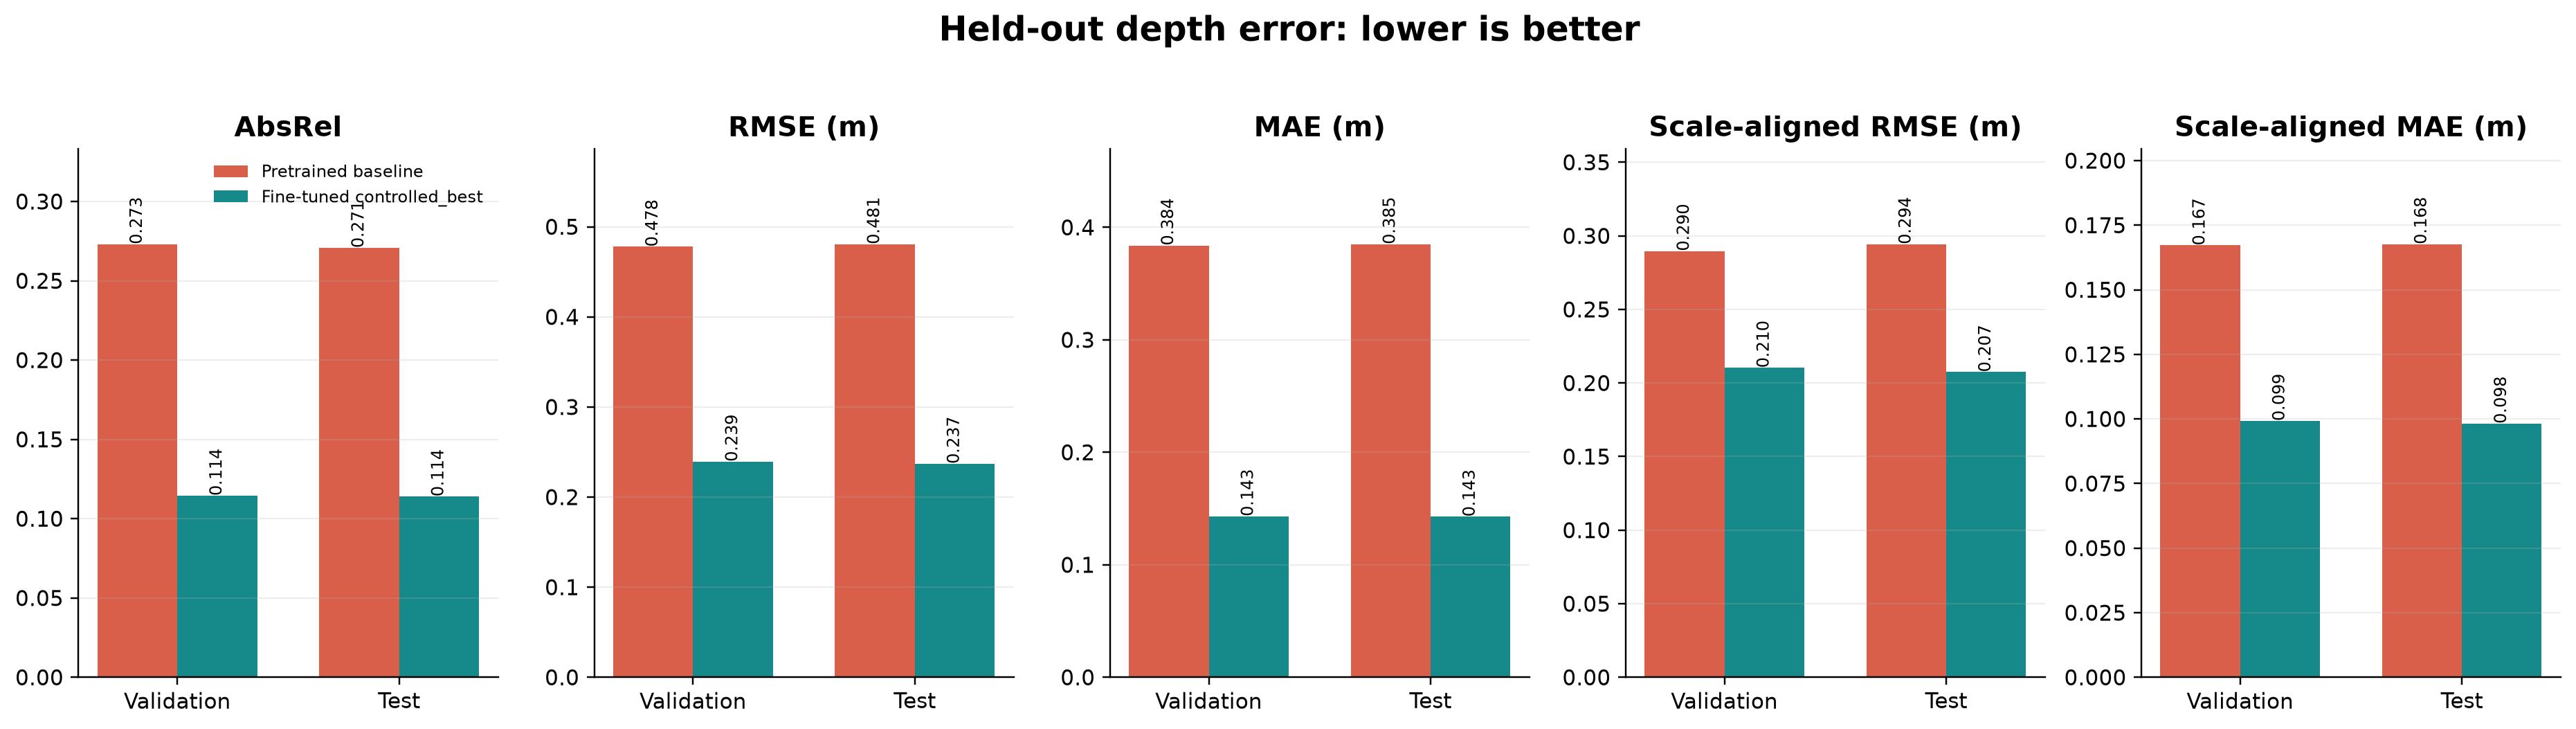
\includegraphics[width=\linewidth]{Run37_eval_error_metrics.png}
        \caption{Các metric lỗi depth trên validation/test.}
    \end{subfigure}
    \vspace{0.35cm}
    \begin{subfigure}{0.78\linewidth}
        \centering
        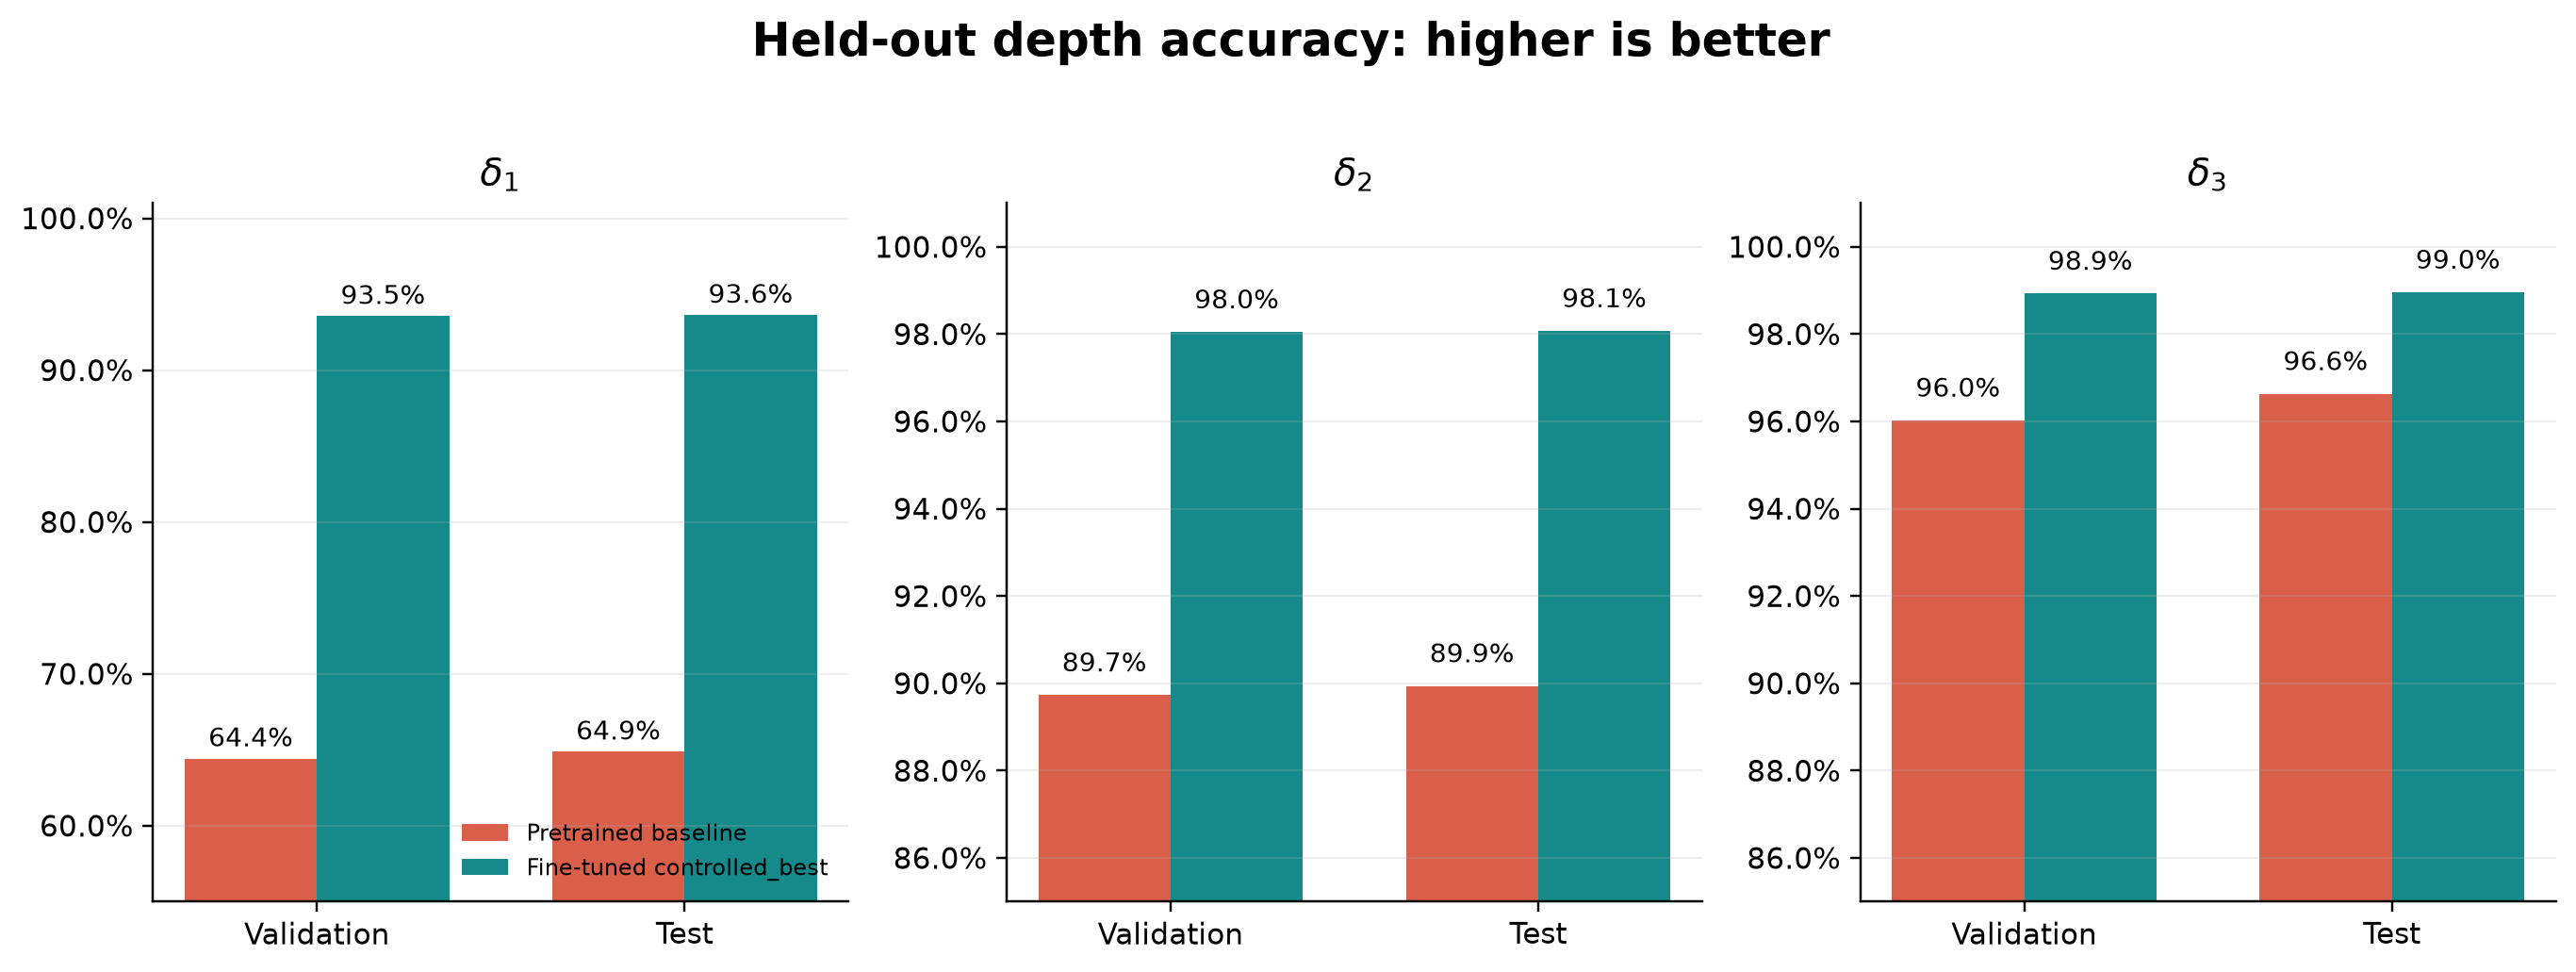
\includegraphics[width=\linewidth]{Run37_eval_accuracy_metrics.png}
        \caption{Các metric accuracy $\delta_1$, $\delta_2$, $\delta_3$.}
    \end{subfigure}
    \caption{So sánh checkpoint pretrained và checkpoint \texttt{controlled\_best} sau fine-tuning.}
    \label{fig:run37_eval_metrics}
\end{figure}

\begin{figure}[H]
    \centering
    \begin{subfigure}{0.92\linewidth}
        \centering
        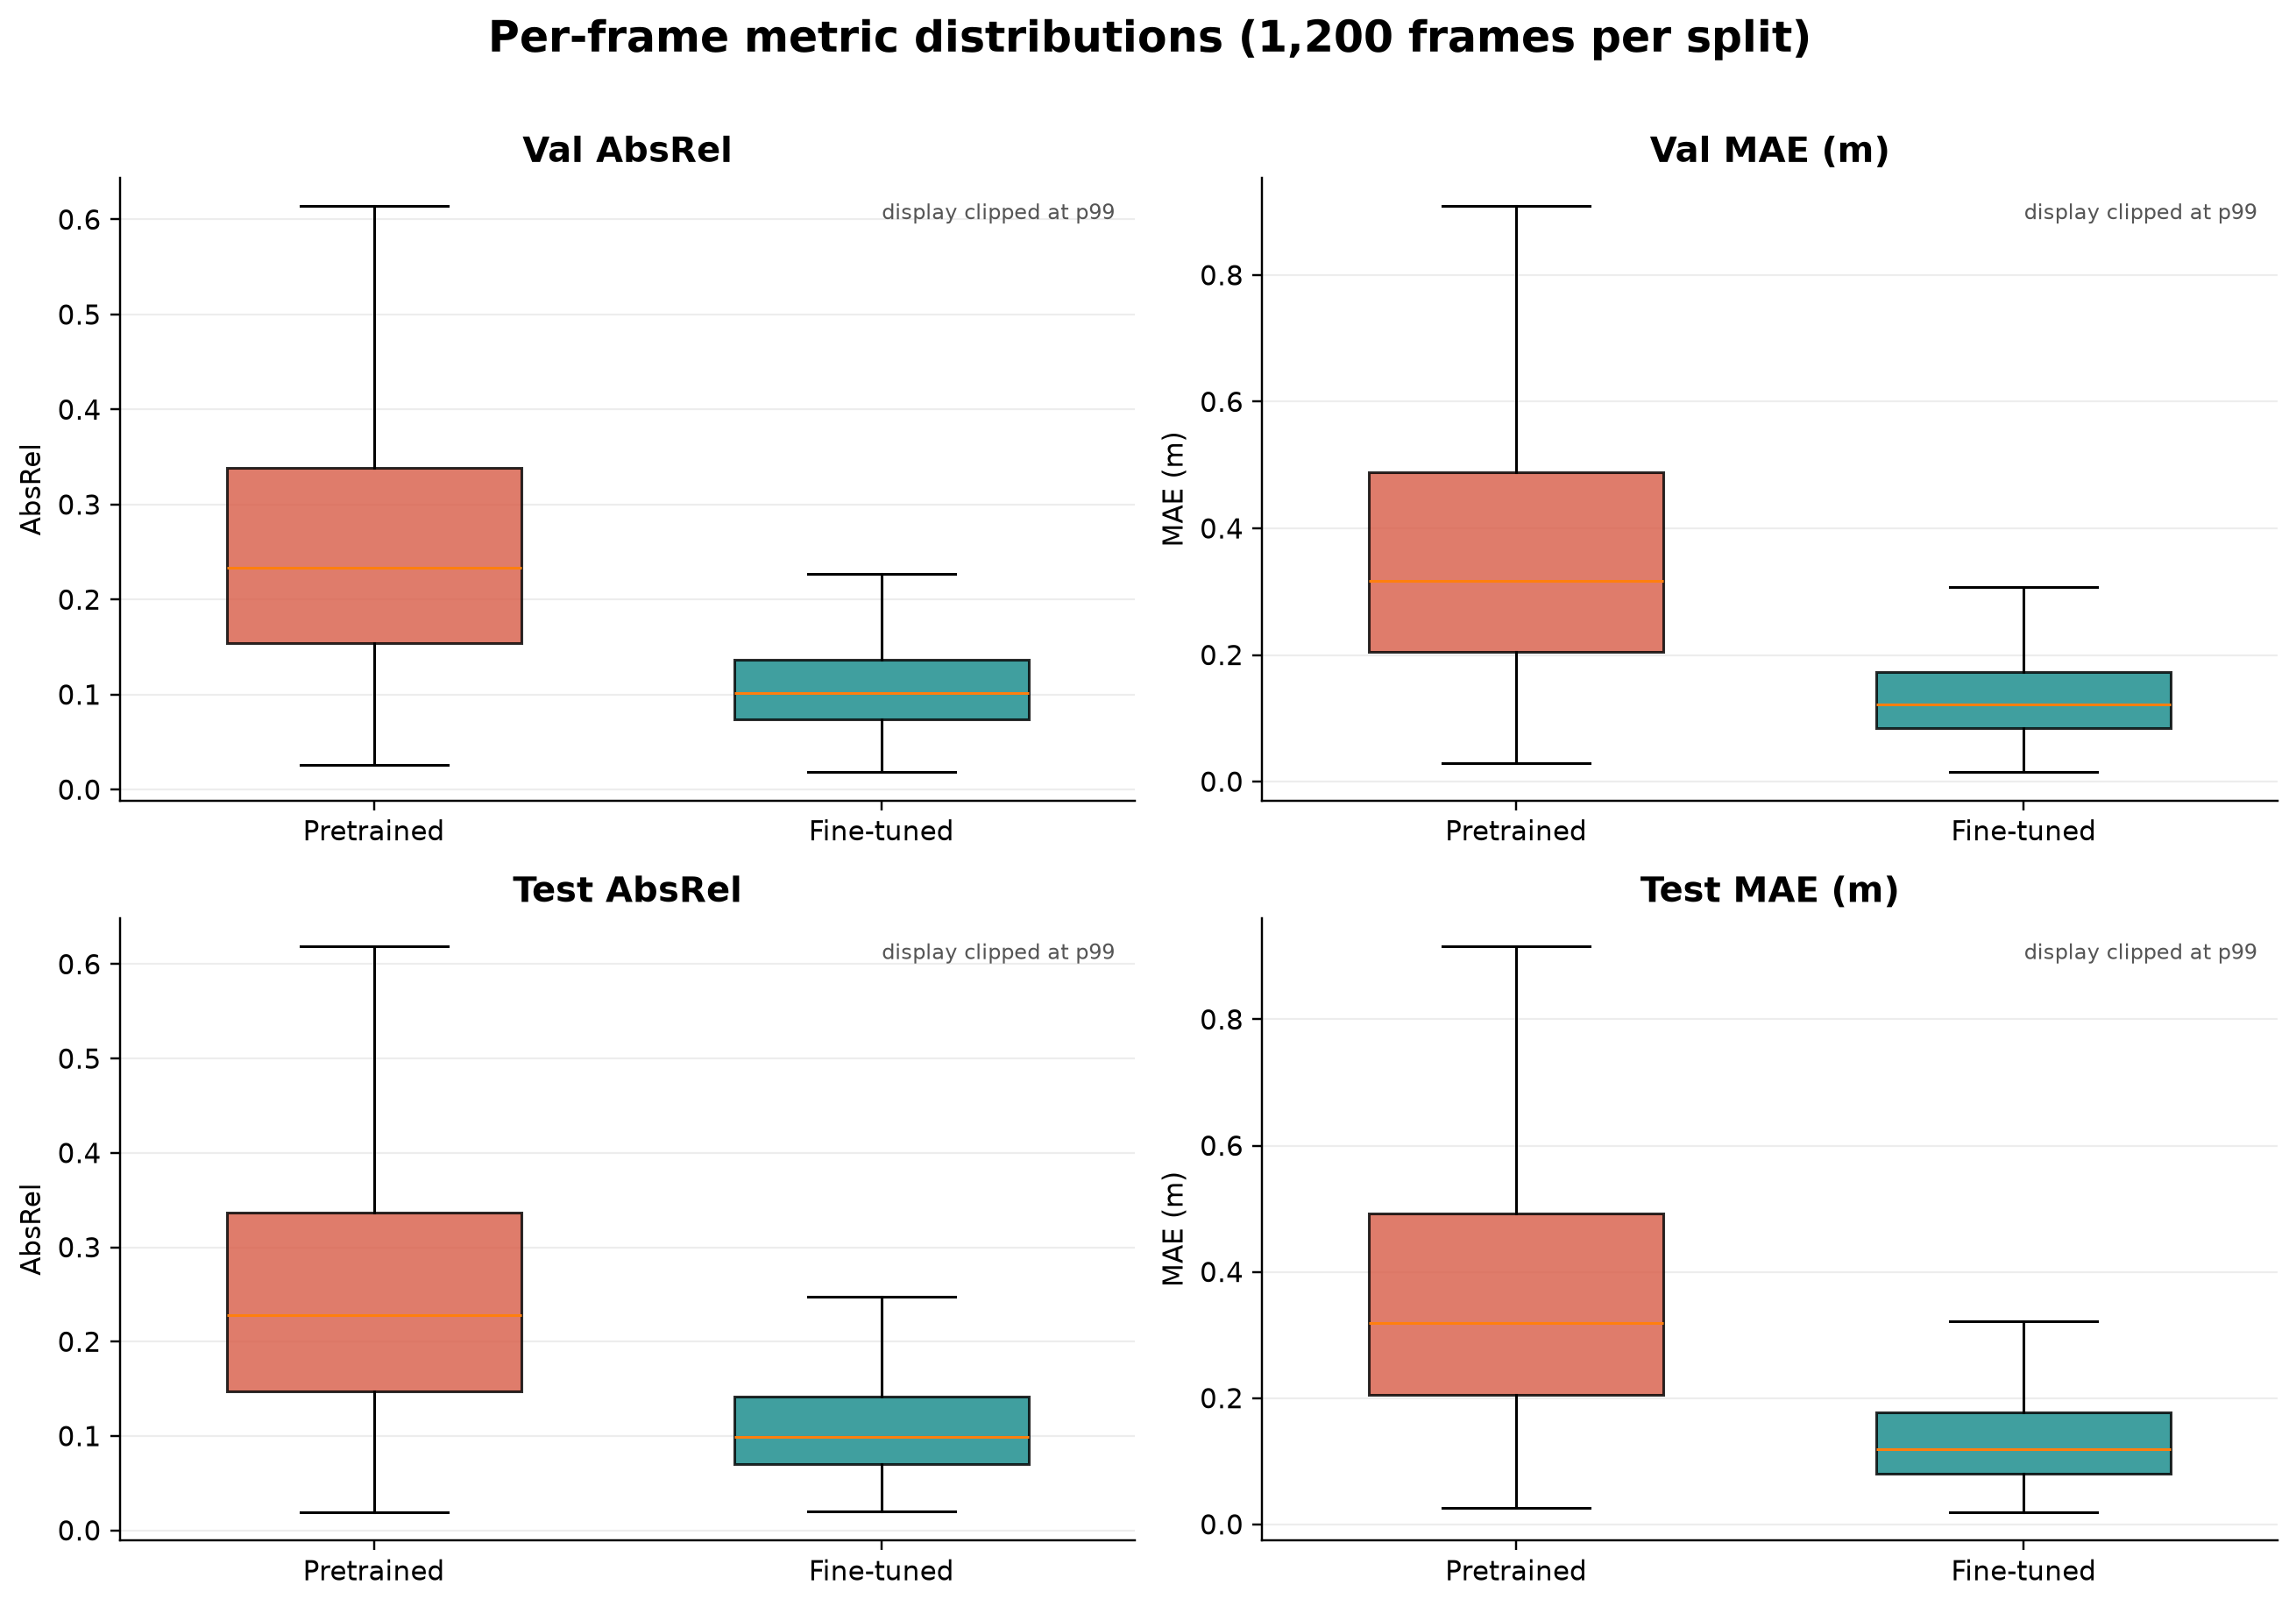
\includegraphics[width=\linewidth]{Run37_per_frame_distributions.png}
        \caption{Phân phối per-frame của các metric depth.}
    \end{subfigure}
    \vspace{0.35cm}
    \begin{subfigure}{0.82\linewidth}
        \centering
        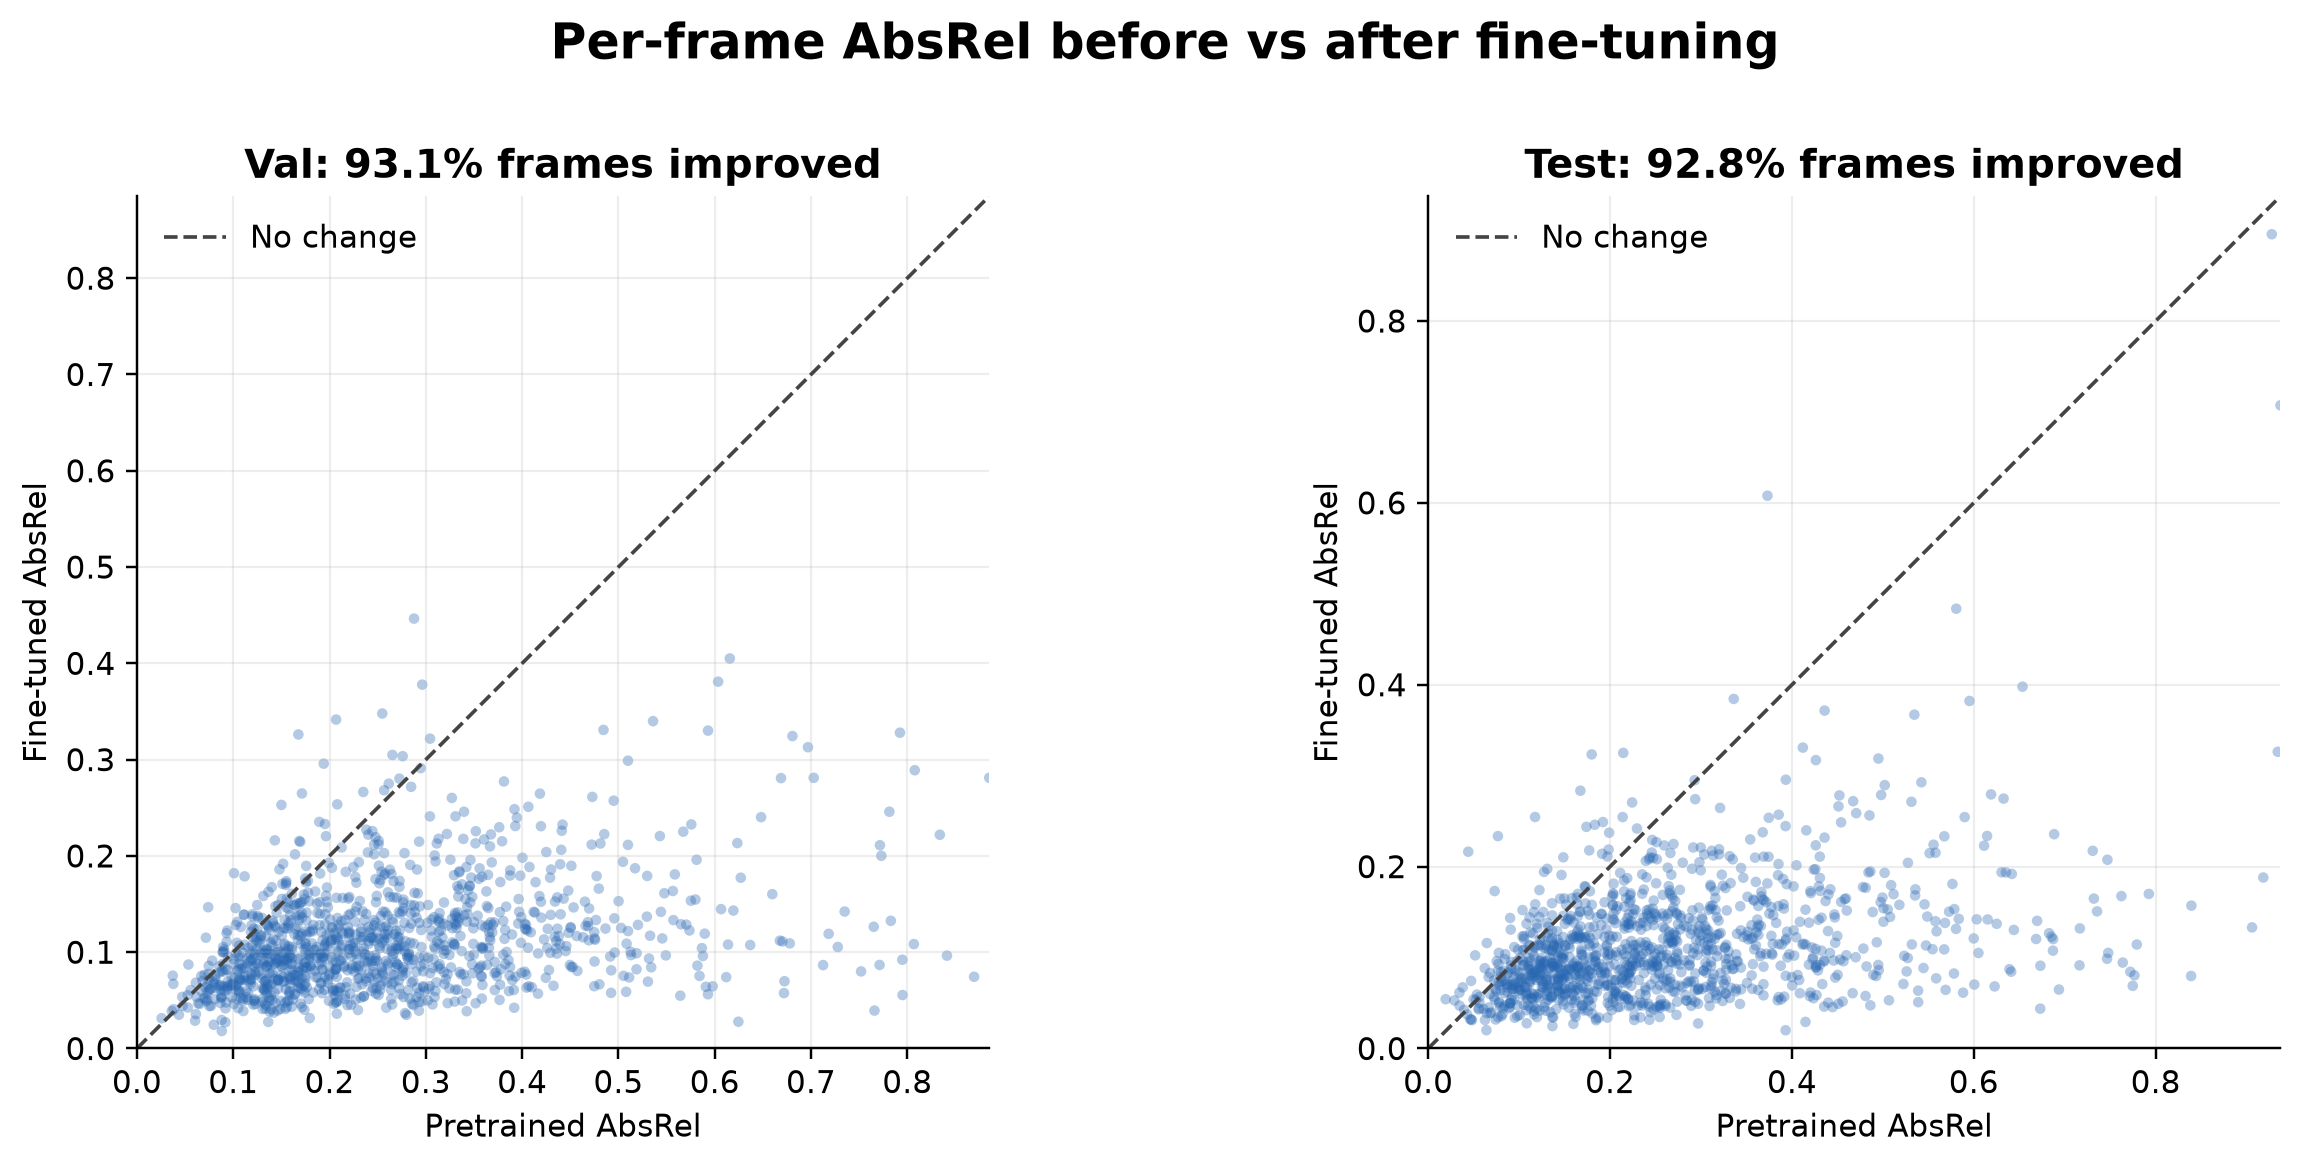
\includegraphics[width=\linewidth]{Run37_absrel_scatter.png}
        \caption{Scatter AbsRel trước và sau fine-tuning.}
    \end{subfigure}
    \caption{Phân tích per-frame cho thấy cải thiện không chỉ đến từ một vài frame dễ. Fine-tuned checkpoint giảm AbsRel trên khoảng 93.1\% validation frames và 92.8\% test frames.}
    \label{fig:run37_per_frame}
\end{figure}

\subsection{Đánh giá tái dựng 3D}
Thí nghiệm tái dựng chính đánh giá liệu hiệu chỉnh bằng độ sâu ước lượng có cải thiện so với RGB-only \mvdp{} hay không. Bảng~\ref{tab:recon} báo cáo Run 41 cached evaluation đã hoàn tất, trong đó tận dụng cached reconstruction records từ Run 38 và Run 39 mà không chạy lại \mvdp{} hoặc depth estimator. Hàng RGB-D đo thật vẫn là mốc oracle từ Run 30. Các số này dùng controlled sparse-view protocol của project, không phải official full ScanNet hoặc ScanNet++ benchmark.

\begin{table}[H]
\centering
\small
\renewcommand{\arraystretch}{1.18}
\resizebox{\linewidth}{!}{%
\begin{tabular}{@{}lcccccc@{}}
\toprule
Phương pháp & Accuracy $\downarrow$ & Completeness $\downarrow$ & Precision $\uparrow$ & Recall $\uparrow$ & F-score $\uparrow$ & Chamfer $\downarrow$ \\
\midrule
RGB-only \mvdp{} & 0.1232 & 0.1571 & 0.2915 & 0.1449 & 0.1929 & 0.2803 \\
Backprojection trực tiếp từ độ sâu ước lượng & 0.1132 & 0.1037 & 0.3542 & 0.2407 & 0.2862 & 0.2170 \\
Hiệu chỉnh bằng độ sâu pretrained & 0.1648 & 0.1558 & 0.1963 & 0.1356 & 0.1600 & 0.3207 \\
Hiệu chỉnh bằng độ sâu đo thật RGB-D & 0.1272 & 0.1385 & 0.3622 & 0.2283 & 0.2745 & 0.2656 \\
Hiệu chỉnh bằng độ sâu ước lượng đã tinh chỉnh (Ours) & 0.1422 & 0.1323 & 0.2368 & 0.1445 & 0.1780 & 0.2745 \\
\bottomrule
\end{tabular}%
}
\caption{So sánh tái dựng 3D từ Run 41 cached evaluation đã hoàn tất. Hàng RGB-D đo thật là mốc tham chiếu/oracle từ Run 30 trong controlled setting, không phải setting triển khai RGB-only.}
\label{tab:recon}
\end{table}

Câu hỏi chính là liệu phương pháp đề xuất có cải thiện so với RGB-only \mvdp{} hay không. Trên subset cached của Run 41, backprojection trực tiếp từ độ sâu ước lượng đã tinh chỉnh đạt F-score và Chamfer tốt nhất, còn hiệu chỉnh bằng độ sâu ước lượng đã tinh chỉnh chưa vượt RGB-only \mvdp{} baseline. Hàng RGB-D đo thật chỉ nên được xem là mốc oracle cho thấy cơ chế correction có thể đạt gì khi dùng depth đo thật.

\subsection{Ablation Study}
Ablation study cần trả lời ba câu hỏi. Thứ nhất, so sánh RGB-only \mvdp{} với hiệu chỉnh bằng độ sâu pretrained cho thấy liệu monocular depth off-the-shelf có giúp ích khi chưa có thích nghi theo task hay không. Thứ hai, so sánh hiệu chỉnh bằng độ sâu pretrained với hiệu chỉnh bằng độ sâu ước lượng đã tinh chỉnh cho thấy việc fine-tuning trên RGB-D training split có cải thiện reconstruction hay không. Thứ ba, so sánh fine-tuned correction với backprojection trực tiếp từ độ sâu ước lượng cho thấy liệu \mvdp{} vẫn đóng góp multi-view geometry hữu ích vượt ngoài bộ ước lượng độ sâu hay không.

Phân tích này quan trọng vì pipeline được đề xuất không đơn thuần là một dự án depth-estimation. Đây là một pipeline tái dựng sử dụng estimated depth để hiệu chỉnh candidate geometry multi-view.

\subsection{Phân tích định tính}
Kết quả định tính nên bao gồm các trực quan hóa point cloud tái dựng đặt cạnh nhau. Với mỗi nhóm scene được chọn, báo cáo nên trình bày: các input RGB views, point cloud RGB-only \mvdp{}, point cloud từ direct estimated-depth, và point cloud cuối cùng sau hiệu chỉnh bằng estimated depth đã tinh chỉnh.

Các ví dụ thành công được kỳ vọng cho thấy ít floating points hơn, bề mặt được căn chỉnh tốt hơn và hình học ổn định hơn trong các vùng mơ hồ. Các failure cases cũng cần được báo cáo, đặc biệt là các scene có occlusion nặng, đồ nội thất lặp lại, bề mặt phản xạ hoặc estimated depth không chính xác.

% ------------------------------------------------------------------
\section{Thảo luận}
Mục tiêu của dự án được đề xuất xuất phát từ tính thực tế khi triển khai. Một hệ thống yêu cầu độ sâu tại thời điểm suy luận có thể chính xác, nhưng nó bị giới hạn vào người dùng có cảm biến chuyên dụng. Một hệ thống chỉ dùng ảnh RGB dễ triển khai hơn vì hầu hết camera mặc định tạo ra ảnh RGB. Vì vậy, dự án sử dụng dữ liệu RGB-D để huấn luyện và đánh giá mô hình, đồng thời giữ đầu vào suy luận cuối cùng là RGB-only.

Thiết kế này cũng thay đổi cách diễn giải dataset. Các depth maps trong dataset không bị bỏ qua. Chúng được dùng làm giám sát để dạy bộ ước lượng độ sâu và làm tham chiếu để đo chất lượng reconstruction. Sản phẩm cuối sau đó áp dụng tri thức độ sâu đã học này lên ảnh đầu vào chỉ có RGB.

Lợi ích kỳ vọng của phương pháp được đề xuất so với RGB-only \mvdp{} là ổn định hình học. \mvdp{} cung cấp candidate geometry multi-view, nhưng vẫn có thể dự đoán wrong-depth trong setting sparse views. Bộ ước lượng độ sâu đã tinh chỉnh cung cấp prior hình học theo từng ảnh. Khi estimated depth đáng tin cậy, module correction có thể kéo candidate points về các vị trí metric hợp lý hơn. Khi estimated depth không đáng tin cậy, correction nên yếu đi hoặc bị từ chối. Điều này tạo động lực cho hướng nghiên cứu tiếp theo về confidence-aware depth correction.

Hạn chế chính là monocular depth vẫn chưa hoàn hảo. Fine-tuning có thể giảm domain mismatch, nhưng không loại bỏ toàn bộ ambiguity. Mô hình vẫn có thể thất bại trong các layout bất thường, vật thể trong suốt, bề mặt phản xạ và các scene có scale khác với phân phối huấn luyện. Vì vậy, claim cuối cùng nên được giới hạn trong đánh giá sparse-view RGB-only có kiểm soát và không nên được trình bày như một official ScanNet benchmark đầy đủ trừ khi giao thức benchmark đầy đủ đã được triển khai.

% ------------------------------------------------------------------
\section{Kết luận}
Dự án này nghiên cứu tái dựng cảnh 3D sparse-view chỉ dùng RGB từ một số lượng nhỏ ảnh 2D thông thường. Động lực mang tính thực tế: phần lớn ảnh đời thường không có độ sâu đo trực tiếp, và việc yêu cầu cảm biến độ sâu sẽ làm giảm phạm vi ứng dụng của hệ thống. Vì vậy, dự án sử dụng dữ liệu RGB-D đo trực tiếp cho giám sát và đánh giá, nhưng không dùng nó làm đầu vào suy luận.

Pipeline được đề xuất kết hợp \mvdp{} với một bộ ước lượng độ sâu monocular đã tinh chỉnh. \mvdp{} tạo ra candidate multi-view geometry từ các ảnh RGB thưa, trong khi bộ ước lượng độ sâu dự đoán pseudo-depth maps từ chính các đầu vào RGB đó. Module hiệu chỉnh bằng estimated depth sau đó tinh chỉnh candidate geometry để giảm lỗi wrong-depth và cải thiện chất lượng point cloud.

Báo cáo định nghĩa một framework đánh giá hoàn chỉnh cho setting này. Chất lượng depth được đo bằng các monocular depth metrics, còn chất lượng tái dựng 3D được đo bằng các point-cloud metrics như accuracy, completeness, precision, recall, F-score và Chamfer distance. So sánh chính là với RGB-only \mvdp{}, direct estimated-depth backprojection và pretrained-depth correction. Phương pháp fine-tuned cuối cùng chỉ nên được chọn nếu nó cải thiện các reconstruction metrics trong ràng buộc suy luận chỉ dùng RGB.

Công việc tiếp theo nên đánh giá thêm nhiều nhóm sparse-view dưới giao thức camera-geometry cập nhật, thêm cơ chế confidence-aware correction và kiểm thử phương pháp trên các tập ảnh RGB thực tế đa dạng hơn. Mục tiêu dài hạn là một hệ thống tái dựng có thể triển khai được, có khả năng tạo hình học cảnh 3D hữu ích từ chỉ một vài ảnh 2D thông thường.

% ------------------------------------------------------------------
\newpage
\begin{thebibliography}{99}
\bibitem{mvdust3r_paper} Z. Tang, Y. Fan, D. Wang, H. Xu, R. Ranjan, A. Schwing, and Z. Yan, ``MV-DUSt3R+: Single-Stage Scene Reconstruction from Sparse Views in 2 Seconds,'' \textit{CVPR}, 2025. Available: \url{https://openaccess.thecvf.com/content/CVPR2025/papers/Tang_MV-DUSt3R_Single-Stage_Scene_Reconstruction_from_Sparse_Views_In_2_Seconds_CVPR_2025_paper.pdf}
\bibitem{mvdust3r_project} Meta Reality Labs, ``MV-DUSt3R+ official implementation,'' GitHub. Available: \url{https://github.com/facebookresearch/mvdust3r}
\bibitem{dust3r_paper} S. Wang, V. Leroy, Y. Cabon, B. Chidlovskii, and J. Revaud, ``DUSt3R: Geometric 3D Vision Made Easy,'' \textit{CVPR}, 2024. Available: \url{https://arxiv.org/abs/2312.14132}
\bibitem{mast3r_paper} V. Leroy, Y. Cabon, and J. Revaud, ``Grounding Image Matching in 3D with MASt3R,'' 2024. Available: \url{https://arxiv.org/abs/2406.09756}
\bibitem{depthanything_project} L. Yang et al., ``Depth Anything V2,'' \textit{NeurIPS}, 2024. Project page: \url{https://depth-anything-v2.github.io/}
\bibitem{depthanything_metric} Depth Anything V2, ``Metric depth estimation README,'' GitHub. Available: \url{https://github.com/depthanything/depth-anything-v2/blob/main/metric_depth/README.md}
\bibitem{scannet} A. Dai, A. X. Chang, M. Savva, M. Halber, T. Funkhouser, and M. Nießner, ``ScanNet: Richly-annotated 3D Reconstructions of Indoor Scenes,'' \textit{CVPR}, 2017. Dataset page: \url{https://www.scan-net.org/ScanNet/}
\bibitem{rsa_depth} Z. Zeng et al., ``RSA: Resolving Scale Ambiguities in Monocular Depth Estimators through Language Descriptions,'' arXiv:2410.02924, 2024. Available: \url{https://arxiv.org/abs/2410.02924}
\bibitem{mde_survey} C. Zhao, Q. Sun, C. Zhang, Y. Tang, and F. Qian, ``Monocular Depth Estimation Based On Deep Learning: An Overview,'' arXiv:2003.06620, 2020. Available: \url{https://arxiv.org/abs/2003.06620}
\end{thebibliography}

\end{document}
